\documentclass[twoside]{book}

% Packages required by doxygen
\usepackage{fixltx2e}
\usepackage{calc}
\usepackage{doxygen}
\usepackage[export]{adjustbox} % also loads graphicx
\usepackage{graphicx}
\usepackage[utf8]{inputenc}
\usepackage{makeidx}
\usepackage{multicol}
\usepackage{multirow}
\PassOptionsToPackage{warn}{textcomp}
\usepackage{textcomp}
\usepackage[nointegrals]{wasysym}
\usepackage[table]{xcolor}

% Font selection
\usepackage[T1]{fontenc}
\usepackage[scaled=.90]{helvet}
\usepackage{courier}
\usepackage{amssymb}
\usepackage{sectsty}
\renewcommand{\familydefault}{\sfdefault}
\allsectionsfont{%
  \fontseries{bc}\selectfont%
  \color{darkgray}%
}
\renewcommand{\DoxyLabelFont}{%
  \fontseries{bc}\selectfont%
  \color{darkgray}%
}
\newcommand{\+}{\discretionary{\mbox{\scriptsize$\hookleftarrow$}}{}{}}

% Page & text layout
\usepackage{geometry}
\geometry{%
  a4paper,%
  top=2.5cm,%
  bottom=2.5cm,%
  left=2.5cm,%
  right=2.5cm%
}
\tolerance=750
\hfuzz=15pt
\hbadness=750
\setlength{\emergencystretch}{15pt}
\setlength{\parindent}{0cm}
\setlength{\parskip}{3ex plus 2ex minus 2ex}
\makeatletter
\renewcommand{\paragraph}{%
  \@startsection{paragraph}{4}{0ex}{-1.0ex}{1.0ex}{%
    \normalfont\normalsize\bfseries\SS@parafont%
  }%
}
\renewcommand{\subparagraph}{%
  \@startsection{subparagraph}{5}{0ex}{-1.0ex}{1.0ex}{%
    \normalfont\normalsize\bfseries\SS@subparafont%
  }%
}
\makeatother

% Headers & footers
\usepackage{fancyhdr}
\pagestyle{fancyplain}
\fancyhead[LE]{\fancyplain{}{\bfseries\thepage}}
\fancyhead[CE]{\fancyplain{}{}}
\fancyhead[RE]{\fancyplain{}{\bfseries\leftmark}}
\fancyhead[LO]{\fancyplain{}{\bfseries\rightmark}}
\fancyhead[CO]{\fancyplain{}{}}
\fancyhead[RO]{\fancyplain{}{\bfseries\thepage}}
\fancyfoot[LE]{\fancyplain{}{}}
\fancyfoot[CE]{\fancyplain{}{}}
\fancyfoot[RE]{\fancyplain{}{\bfseries\scriptsize Generated by Doxygen }}
\fancyfoot[LO]{\fancyplain{}{\bfseries\scriptsize Generated by Doxygen }}
\fancyfoot[CO]{\fancyplain{}{}}
\fancyfoot[RO]{\fancyplain{}{}}
\renewcommand{\footrulewidth}{0.4pt}
\renewcommand{\chaptermark}[1]{%
  \markboth{#1}{}%
}
\renewcommand{\sectionmark}[1]{%
  \markright{\thesection\ #1}%
}

% Indices & bibliography
\usepackage{natbib}
\usepackage[titles]{tocloft}
\setcounter{tocdepth}{3}
\setcounter{secnumdepth}{5}
\makeindex

% Hyperlinks (required, but should be loaded last)
\usepackage{ifpdf}
\ifpdf
  \usepackage[pdftex,pagebackref=true]{hyperref}
\else
  \usepackage[ps2pdf,pagebackref=true]{hyperref}
\fi
\hypersetup{%
  colorlinks=true,%
  linkcolor=blue,%
  citecolor=blue,%
  unicode%
}

% Custom commands
\newcommand{\clearemptydoublepage}{%
  \newpage{\pagestyle{empty}\cleardoublepage}%
}

\usepackage{caption}
\captionsetup{labelsep=space,justification=centering,font={bf},singlelinecheck=off,skip=4pt,position=top}

%===== C O N T E N T S =====

\begin{document}

% Titlepage & ToC
\hypersetup{pageanchor=false,
             bookmarksnumbered=true,
             pdfencoding=unicode
            }
\pagenumbering{alph}
\begin{titlepage}
\vspace*{7cm}
\begin{center}%
{\Large My Project }\\
\vspace*{1cm}
{\large Generated by Doxygen 1.8.14}\\
\end{center}
\end{titlepage}
\clearemptydoublepage
\pagenumbering{roman}
\tableofcontents
\clearemptydoublepage
\pagenumbering{arabic}
\hypersetup{pageanchor=true}

%--- Begin generated contents ---
\chapter{Hierarchical Index}
\section{Class Hierarchy}
This inheritance list is sorted roughly, but not completely, alphabetically\+:\begin{DoxyCompactList}
\item \contentsline{section}{g\+Sparse\+:\+:ER\+:\+:Policy\+:\+:Aprox\+E\+R\+S\+L\+M\+Jacobi\+CG}{\pageref{classg_sparse_1_1_e_r_1_1_policy_1_1_aprox_e_r_s_l_m_jacobi_c_g}}{}
\item \contentsline{section}{g\+Sparse\+:\+:ER\+:\+:Policy\+:\+:Exact\+E\+R\+Jacobi\+CG}{\pageref{classg_sparse_1_1_e_r_1_1_policy_1_1_exact_e_r_jacobi_c_g}}{}
\item \contentsline{section}{g\+Sparse\+:\+:I\+Effective\+Resistance}{\pageref{classg_sparse_1_1_i_effective_resistance}}{}
\begin{DoxyCompactList}
\item \contentsline{section}{g\+Sparse\+:\+:ER\+:\+:\+\_\+\+Approximate\+ER$<$ Policy $>$}{\pageref{classg_sparse_1_1_e_r_1_1___approximate_e_r}}{}
\item \contentsline{section}{g\+Sparse\+:\+:ER\+:\+:\+\_\+\+Exact\+ER$<$ Policy $>$}{\pageref{classg_sparse_1_1_e_r_1_1___exact_e_r}}{}
\end{DoxyCompactList}
\item \contentsline{section}{g\+Sparse\+:\+:I\+Graph}{\pageref{classg_sparse_1_1_i_graph}}{}
\begin{DoxyCompactList}
\item \contentsline{section}{g\+Sparse\+:\+:Undirected\+Graph}{\pageref{classg_sparse_1_1_undirected_graph}}{}
\end{DoxyCompactList}
\item \contentsline{section}{g\+Sparse\+:\+:I\+Graph\+Reader}{\pageref{classg_sparse_1_1_i_graph_reader}}{}
\begin{DoxyCompactList}
\item \contentsline{section}{g\+Sparse\+:\+:Graph\+C\+S\+V\+Reader}{\pageref{classg_sparse_1_1_graph_c_s_v_reader}}{}
\end{DoxyCompactList}
\item \contentsline{section}{g\+Sparse\+:\+:I\+Graph\+Writer}{\pageref{classg_sparse_1_1_i_graph_writer}}{}
\begin{DoxyCompactList}
\item \contentsline{section}{g\+Sparse\+:\+:Graph\+C\+S\+V\+Writer}{\pageref{classg_sparse_1_1_graph_c_s_v_writer}}{}
\end{DoxyCompactList}
\item \contentsline{section}{g\+Sparse\+:\+:I\+Sparsifier}{\pageref{classg_sparse_1_1_i_sparsifier}}{}
\begin{DoxyCompactList}
\item \contentsline{section}{g\+Sparse\+:\+:Spectral\+Sparsifier\+:\+:E\+R\+Sampling}{\pageref{classg_sparse_1_1_spectral_sparsifier_1_1_e_r_sampling}}{}
\end{DoxyCompactList}
\item Policy\begin{DoxyCompactList}
\item \contentsline{section}{g\+Sparse\+:\+:ER\+:\+:\+\_\+\+Approximate\+ER$<$ Policy $>$}{\pageref{classg_sparse_1_1_e_r_1_1___approximate_e_r}}{}
\item \contentsline{section}{g\+Sparse\+:\+:ER\+:\+:\+\_\+\+Exact\+ER$<$ Policy $>$}{\pageref{classg_sparse_1_1_e_r_1_1___exact_e_r}}{}
\end{DoxyCompactList}
\end{DoxyCompactList}

\chapter{Class Index}
\section{Class List}
Here are the classes, structs, unions and interfaces with brief descriptions\+:\begin{DoxyCompactList}
\item\contentsline{section}{\mbox{\hyperlink{class_library_1_1v1_1_1_q_tstyle___test}{Library\+::v1\+::\+Q\+Tstyle\+\_\+\+Test}} \\*A test class }{\pageref{class_library_1_1v1_1_1_q_tstyle___test}}{}
\end{DoxyCompactList}

\chapter{Class Documentation}
\hypertarget{classg_sparse_1_1_e_r_1_1___approximate_e_r}{}\section{g\+Sparse\+:\+:ER\+:\+:\+\_\+\+Approximate\+ER$<$ Policy $>$ Class Template Reference}
\label{classg_sparse_1_1_e_r_1_1___approximate_e_r}\index{g\+Sparse\+::\+E\+R\+::\+\_\+\+Approximate\+E\+R$<$ Policy $>$@{g\+Sparse\+::\+E\+R\+::\+\_\+\+Approximate\+E\+R$<$ Policy $>$}}
Inheritance diagram for g\+Sparse\+:\+:ER\+:\+:\+\_\+\+Approximate\+ER$<$ Policy $>$\+:\begin{figure}[H]
\begin{center}
\leavevmode
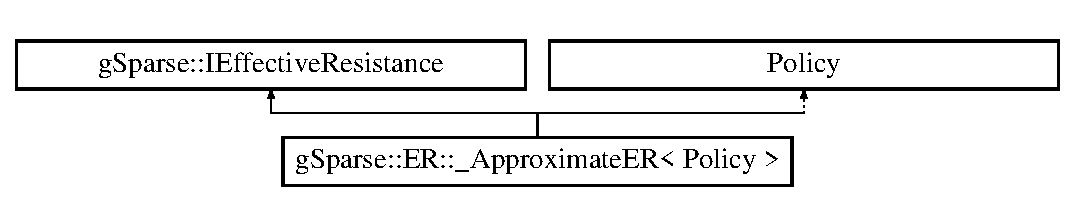
\includegraphics[height=2.000000cm]{classg_sparse_1_1_e_r_1_1___approximate_e_r}
\end{center}
\end{figure}
\subsection*{Public Member Functions}
\begin{DoxyCompactItemize}
\item 
\mbox{\Hypertarget{classg_sparse_1_1_e_r_1_1___approximate_e_r_abf16cea687d1129e1a13b4af0db44892}\label{classg_sparse_1_1_e_r_1_1___approximate_e_r_abf16cea687d1129e1a13b4af0db44892}} 
g\+Sparse\+::\+C\+O\+M\+P\+U\+T\+E\+\_\+\+I\+N\+FO \mbox{\hyperlink{classg_sparse_1_1_e_r_1_1___approximate_e_r_abf16cea687d1129e1a13b4af0db44892}{Calculate\+ER}} (g\+Sparse\+::\+Precision\+Row\+Matrix \&er, const g\+Sparse\+::\+Graph \&graph)
\begin{DoxyCompactList}\small\item\em A pure virtual member to computer sparsifier weight. \end{DoxyCompactList}\end{DoxyCompactItemize}


The documentation for this class was generated from the following file\+:\begin{DoxyCompactItemize}
\item 
/\+Users/\+Bomb/\+Documents/\+Project/g\+Sparse/include/g\+Sparse/\+E\+R/Approximate\+E\+R.\+hpp\end{DoxyCompactItemize}

\hypertarget{classg_sparse_1_1_e_r_1_1___exact_e_r}{}\section{g\+Sparse\+:\+:ER\+:\+:\+\_\+\+Exact\+ER$<$ Policy $>$ Class Template Reference}
\label{classg_sparse_1_1_e_r_1_1___exact_e_r}\index{g\+Sparse\+::\+E\+R\+::\+\_\+\+Exact\+E\+R$<$ Policy $>$@{g\+Sparse\+::\+E\+R\+::\+\_\+\+Exact\+E\+R$<$ Policy $>$}}
Inheritance diagram for g\+Sparse\+:\+:ER\+:\+:\+\_\+\+Exact\+ER$<$ Policy $>$\+:\begin{figure}[H]
\begin{center}
\leavevmode
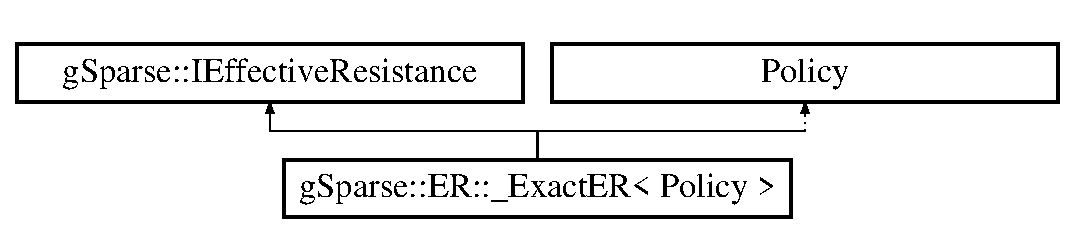
\includegraphics[height=2.000000cm]{classg_sparse_1_1_e_r_1_1___exact_e_r}
\end{center}
\end{figure}
\subsection*{Public Member Functions}
\begin{DoxyCompactItemize}
\item 
\mbox{\Hypertarget{classg_sparse_1_1_e_r_1_1___exact_e_r_a47b950a81c815626a9d51a6284d1d49d}\label{classg_sparse_1_1_e_r_1_1___exact_e_r_a47b950a81c815626a9d51a6284d1d49d}} 
g\+Sparse\+::\+C\+O\+M\+P\+U\+T\+E\+\_\+\+I\+N\+FO \mbox{\hyperlink{classg_sparse_1_1_e_r_1_1___exact_e_r_a47b950a81c815626a9d51a6284d1d49d}{Calculate\+ER}} (g\+Sparse\+::\+Precision\+Row\+Matrix \&er, const g\+Sparse\+::\+Graph \&graph)
\begin{DoxyCompactList}\small\item\em A pure virtual member to computer sparsifier weight. \end{DoxyCompactList}\end{DoxyCompactItemize}


The documentation for this class was generated from the following file\+:\begin{DoxyCompactItemize}
\item 
/\+Users/\+Bomb/\+Documents/\+Project/g\+Sparse/include/g\+Sparse/\+E\+R/Exact\+E\+R.\+hpp\end{DoxyCompactItemize}

\hypertarget{classg_sparse_1_1_e_r_1_1_policy_1_1_aprox_e_r_s_l_m_jacobi_c_g}{}\section{g\+Sparse\+:\+:ER\+:\+:Policy\+:\+:Aprox\+E\+R\+S\+L\+M\+Jacobi\+CG Class Reference}
\label{classg_sparse_1_1_e_r_1_1_policy_1_1_aprox_e_r_s_l_m_jacobi_c_g}\index{g\+Sparse\+::\+E\+R\+::\+Policy\+::\+Aprox\+E\+R\+S\+L\+M\+Jacobi\+CG@{g\+Sparse\+::\+E\+R\+::\+Policy\+::\+Aprox\+E\+R\+S\+L\+M\+Jacobi\+CG}}
\subsection*{Protected Member Functions}
\begin{DoxyCompactItemize}
\item 
\mbox{\Hypertarget{classg_sparse_1_1_e_r_1_1_policy_1_1_aprox_e_r_s_l_m_jacobi_c_g_a0174f484153579201e058996a3d19564}\label{classg_sparse_1_1_e_r_1_1_policy_1_1_aprox_e_r_s_l_m_jacobi_c_g_a0174f484153579201e058996a3d19564}} 
g\+Sparse\+::\+C\+O\+M\+P\+U\+T\+E\+\_\+\+I\+N\+FO {\bfseries \+\_\+calculate\+ER} (g\+Sparse\+::\+Precision\+Row\+Matrix \&er, const g\+Sparse\+::\+Graph \&graph, double eps=1.\+0f, double J\+L\+Tol=0.\+5, int max\+Iter=300)
\end{DoxyCompactItemize}


The documentation for this class was generated from the following file\+:\begin{DoxyCompactItemize}
\item 
/\+Users/\+Bomb/\+Documents/\+Project/g\+Sparse/include/g\+Sparse/\+E\+R/\+Policy/Aprox\+E\+R\+S\+L\+M\+Jacobi\+C\+G.\+hpp\end{DoxyCompactItemize}

\hypertarget{classg_sparse_1_1_spectral_sparsifier_1_1_e_r_sampling}{}\section{g\+Sparse\+:\+:Spectral\+Sparsifier\+:\+:E\+R\+Sampling Class Reference}
\label{classg_sparse_1_1_spectral_sparsifier_1_1_e_r_sampling}\index{g\+Sparse\+::\+Spectral\+Sparsifier\+::\+E\+R\+Sampling@{g\+Sparse\+::\+Spectral\+Sparsifier\+::\+E\+R\+Sampling}}


{\ttfamily \#include $<$E\+R\+Sampling.\+hpp$>$}

Inheritance diagram for g\+Sparse\+:\+:Spectral\+Sparsifier\+:\+:E\+R\+Sampling\+:\begin{figure}[H]
\begin{center}
\leavevmode
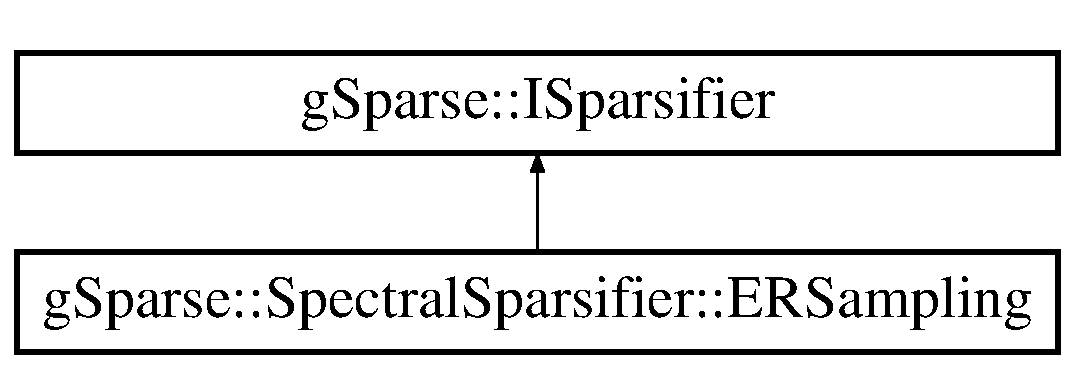
\includegraphics[height=2.000000cm]{classg_sparse_1_1_spectral_sparsifier_1_1_e_r_sampling}
\end{center}
\end{figure}
\subsection*{Public Member Functions}
\begin{DoxyCompactItemize}
\item 
\mbox{\hyperlink{classg_sparse_1_1_spectral_sparsifier_1_1_e_r_sampling_a1ceb48c424600cbe6d315f3f5bad1598}{E\+R\+Sampling}} (const g\+Sparse\+::\+Graph \&graph, double C=4.\+0f, double Epsilon=0.\+3f, g\+Sparse\+::\+Spectral\+Sparsifier\+::\+E\+R\+\_\+\+M\+E\+T\+H\+O\+D\+S E\+R\+Policy=g\+Sparse\+::\+Spectral\+Sparsifier\+::\+A\+P\+P\+R\+O\+X\+I\+M\+A\+T\+E\+\_\+\+E\+R)
\item 
virtual g\+Sparse\+::\+C\+O\+M\+P\+U\+T\+E\+\_\+\+I\+N\+FO \mbox{\hyperlink{classg_sparse_1_1_spectral_sparsifier_1_1_e_r_sampling_a4751e449a9c2fa43b57db6eb703a622d}{Compute}} ()
\item 
virtual g\+Sparse\+::\+Graph \mbox{\hyperlink{classg_sparse_1_1_spectral_sparsifier_1_1_e_r_sampling_a5322f1076777028699d010daa5cd2406}{Get\+Sparsified\+Graph}} ()
\item 
void \mbox{\hyperlink{classg_sparse_1_1_spectral_sparsifier_1_1_e_r_sampling_a35cf40021c7fa90b5dda042896691bff}{Set\+E\+R\+Policy}} (E\+R\+\_\+\+M\+E\+T\+H\+O\+DS policy)
\item 
void \mbox{\hyperlink{classg_sparse_1_1_spectral_sparsifier_1_1_e_r_sampling_a35bf03bbda2e0d37345ce8d460e734a4}{SetC}} (double C)
\item 
void \mbox{\hyperlink{classg_sparse_1_1_spectral_sparsifier_1_1_e_r_sampling_a57eceac9af3b8846c3370eca999a9a57}{Set\+Epsilon}} (double Epsilon)
\item 
\mbox{\Hypertarget{classg_sparse_1_1_spectral_sparsifier_1_1_e_r_sampling_abd617a6dacb79fda563caf6509972667}\label{classg_sparse_1_1_spectral_sparsifier_1_1_e_r_sampling_abd617a6dacb79fda563caf6509972667}} 
double \mbox{\hyperlink{classg_sparse_1_1_spectral_sparsifier_1_1_e_r_sampling_abd617a6dacb79fda563caf6509972667}{GetC}} () const
\begin{DoxyCompactList}\small\item\em Get the sparsifier\textquotesingle{}s current configuration for hyper-\/parameter C. \end{DoxyCompactList}\item 
\mbox{\Hypertarget{classg_sparse_1_1_spectral_sparsifier_1_1_e_r_sampling_a57a513740f9eff3113b518132c60cb0a}\label{classg_sparse_1_1_spectral_sparsifier_1_1_e_r_sampling_a57a513740f9eff3113b518132c60cb0a}} 
double \mbox{\hyperlink{classg_sparse_1_1_spectral_sparsifier_1_1_e_r_sampling_a57a513740f9eff3113b518132c60cb0a}{Get\+Epsilon}} () const
\begin{DoxyCompactList}\small\item\em Get the sparsifier\textquotesingle{}s current configuration for hyper-\/parameter Epsilon. \end{DoxyCompactList}\item 
\mbox{\Hypertarget{classg_sparse_1_1_spectral_sparsifier_1_1_e_r_sampling_a9db84943ae4c2ff370ef59bcdc5c255c}\label{classg_sparse_1_1_spectral_sparsifier_1_1_e_r_sampling_a9db84943ae4c2ff370ef59bcdc5c255c}} 
g\+Sparse\+::\+Spectral\+Sparsifier\+::\+E\+R\+\_\+\+M\+E\+T\+H\+O\+DS \mbox{\hyperlink{classg_sparse_1_1_spectral_sparsifier_1_1_e_r_sampling_a9db84943ae4c2ff370ef59bcdc5c255c}{Get\+E\+R\+Policy}} () const
\begin{DoxyCompactList}\small\item\em Get the sparsifier\textquotesingle{}s current Effective Resistance policy. \end{DoxyCompactList}\item 
\mbox{\Hypertarget{classg_sparse_1_1_spectral_sparsifier_1_1_e_r_sampling_a898a55838f700015cdfa999b2b0fabe8}\label{classg_sparse_1_1_spectral_sparsifier_1_1_e_r_sampling_a898a55838f700015cdfa999b2b0fabe8}} 
g\+Sparse\+::\+C\+O\+M\+P\+U\+T\+E\+\_\+\+I\+N\+FO \mbox{\hyperlink{classg_sparse_1_1_spectral_sparsifier_1_1_e_r_sampling_a898a55838f700015cdfa999b2b0fabe8}{Get\+Info}} () const
\begin{DoxyCompactList}\small\item\em Get the sparsifier\textquotesingle{}s current computation information. \end{DoxyCompactList}\item 
\mbox{\Hypertarget{classg_sparse_1_1_spectral_sparsifier_1_1_e_r_sampling_a4b0ef0dc57feea2b927c86d1cd422273}\label{classg_sparse_1_1_spectral_sparsifier_1_1_e_r_sampling_a4b0ef0dc57feea2b927c86d1cd422273}} 
const g\+Sparse\+::\+Precision\+Row\+Matrix \& \mbox{\hyperlink{classg_sparse_1_1_spectral_sparsifier_1_1_e_r_sampling_a4b0ef0dc57feea2b927c86d1cd422273}{Get\+Effective\+Resistance}} () const
\begin{DoxyCompactList}\small\item\em Get the effective resistance of the graph specified at construction. \end{DoxyCompactList}\end{DoxyCompactItemize}
\subsection*{Protected Attributes}
\begin{DoxyCompactItemize}
\item 
\mbox{\Hypertarget{classg_sparse_1_1_spectral_sparsifier_1_1_e_r_sampling_a0ed4651553939cedd57e217719ce5a81}\label{classg_sparse_1_1_spectral_sparsifier_1_1_e_r_sampling_a0ed4651553939cedd57e217719ce5a81}} 
double \mbox{\hyperlink{classg_sparse_1_1_spectral_sparsifier_1_1_e_r_sampling_a0ed4651553939cedd57e217719ce5a81}{\+\_\+c}}
\begin{DoxyCompactList}\small\item\em C-\/hyper parameter. \end{DoxyCompactList}\item 
\mbox{\Hypertarget{classg_sparse_1_1_spectral_sparsifier_1_1_e_r_sampling_acd8735c70eabe432edefde7ca0c13d19}\label{classg_sparse_1_1_spectral_sparsifier_1_1_e_r_sampling_acd8735c70eabe432edefde7ca0c13d19}} 
double \mbox{\hyperlink{classg_sparse_1_1_spectral_sparsifier_1_1_e_r_sampling_acd8735c70eabe432edefde7ca0c13d19}{\+\_\+eps}}
\begin{DoxyCompactList}\small\item\em epsilon hyper-\/parameter. \end{DoxyCompactList}\item 
\mbox{\Hypertarget{classg_sparse_1_1_spectral_sparsifier_1_1_e_r_sampling_a311f71d4fba0c038b1f2e751859c1a5f}\label{classg_sparse_1_1_spectral_sparsifier_1_1_e_r_sampling_a311f71d4fba0c038b1f2e751859c1a5f}} 
g\+Sparse\+::\+C\+O\+M\+P\+U\+T\+E\+\_\+\+I\+N\+FO \mbox{\hyperlink{classg_sparse_1_1_spectral_sparsifier_1_1_e_r_sampling_a311f71d4fba0c038b1f2e751859c1a5f}{\+\_\+compute\+Info}}
\begin{DoxyCompactList}\small\item\em Status of sparsifier. \end{DoxyCompactList}\item 
\mbox{\Hypertarget{classg_sparse_1_1_spectral_sparsifier_1_1_e_r_sampling_ae6a16bbd5a376677ebddc0c657c0da14}\label{classg_sparse_1_1_spectral_sparsifier_1_1_e_r_sampling_ae6a16bbd5a376677ebddc0c657c0da14}} 
g\+Sparse\+::\+Graph \mbox{\hyperlink{classg_sparse_1_1_spectral_sparsifier_1_1_e_r_sampling_ae6a16bbd5a376677ebddc0c657c0da14}{\+\_\+graph}}
\begin{DoxyCompactList}\small\item\em Graph to Sparsify. \end{DoxyCompactList}\item 
\mbox{\Hypertarget{classg_sparse_1_1_spectral_sparsifier_1_1_e_r_sampling_a54a2bc9c9dfda467a946c64afcfc46fc}\label{classg_sparse_1_1_spectral_sparsifier_1_1_e_r_sampling_a54a2bc9c9dfda467a946c64afcfc46fc}} 
g\+Sparse\+::\+Precision\+Row\+Matrix \mbox{\hyperlink{classg_sparse_1_1_spectral_sparsifier_1_1_e_r_sampling_a54a2bc9c9dfda467a946c64afcfc46fc}{\+\_\+er}}
\begin{DoxyCompactList}\small\item\em Effective Resistance. \end{DoxyCompactList}\item 
\mbox{\Hypertarget{classg_sparse_1_1_spectral_sparsifier_1_1_e_r_sampling_aa6ab4a22339f9846fabc82437dced6f2}\label{classg_sparse_1_1_spectral_sparsifier_1_1_e_r_sampling_aa6ab4a22339f9846fabc82437dced6f2}} 
g\+Sparse\+::\+Effective\+Resistance \mbox{\hyperlink{classg_sparse_1_1_spectral_sparsifier_1_1_e_r_sampling_aa6ab4a22339f9846fabc82437dced6f2}{\+\_\+er\+Calculator}}
\begin{DoxyCompactList}\small\item\em Pointer to Effective\+Resistance module. \end{DoxyCompactList}\item 
\mbox{\Hypertarget{classg_sparse_1_1_spectral_sparsifier_1_1_e_r_sampling_a26b6aebe0adb1851149c74017fdb73e0}\label{classg_sparse_1_1_spectral_sparsifier_1_1_e_r_sampling_a26b6aebe0adb1851149c74017fdb73e0}} 
g\+Sparse\+::\+Spectral\+Sparsifier\+::\+E\+R\+\_\+\+M\+E\+T\+H\+O\+DS \mbox{\hyperlink{classg_sparse_1_1_spectral_sparsifier_1_1_e_r_sampling_a26b6aebe0adb1851149c74017fdb73e0}{\+\_\+er\+Policy}}
\begin{DoxyCompactList}\small\item\em Effective\+Resistance Calculation Policy. \end{DoxyCompactList}\end{DoxyCompactItemize}


\subsection{Detailed Description}
This class implements Spectral Sparsifier by Effective Weight Sampling. Original paper \href{https://arxiv.org/pdf/0803.0929.pdf}{\tt https\+://arxiv.\+org/pdf/0803.\+0929.\+pdf} 

\subsection{Constructor \& Destructor Documentation}
\mbox{\Hypertarget{classg_sparse_1_1_spectral_sparsifier_1_1_e_r_sampling_a1ceb48c424600cbe6d315f3f5bad1598}\label{classg_sparse_1_1_spectral_sparsifier_1_1_e_r_sampling_a1ceb48c424600cbe6d315f3f5bad1598}} 
\index{g\+Sparse\+::\+Spectral\+Sparsifier\+::\+E\+R\+Sampling@{g\+Sparse\+::\+Spectral\+Sparsifier\+::\+E\+R\+Sampling}!E\+R\+Sampling@{E\+R\+Sampling}}
\index{E\+R\+Sampling@{E\+R\+Sampling}!g\+Sparse\+::\+Spectral\+Sparsifier\+::\+E\+R\+Sampling@{g\+Sparse\+::\+Spectral\+Sparsifier\+::\+E\+R\+Sampling}}
\subsubsection{\texorpdfstring{E\+R\+Sampling()}{ERSampling()}}
{\footnotesize\ttfamily g\+Sparse\+::\+Spectral\+Sparsifier\+::\+E\+R\+Sampling\+::\+E\+R\+Sampling (\begin{DoxyParamCaption}\item[{const g\+Sparse\+::\+Graph \&}]{graph,  }\item[{double}]{C = {\ttfamily 4.0f},  }\item[{double}]{Epsilon = {\ttfamily 0.3f},  }\item[{g\+Sparse\+::\+Spectral\+Sparsifier\+::\+E\+R\+\_\+\+M\+E\+T\+H\+O\+DS}]{E\+R\+Policy = {\ttfamily gSparse\+:\+:SpectralSparsifier\+:\+:APPROXIMATE\+\_\+ER} }\end{DoxyParamCaption})\hspace{0.3cm}{\ttfamily [inline]}}

Constructor to create a \mbox{\hyperlink{classg_sparse_1_1_i_sparsifier}{I\+Sparsifier}} object to perform Spectral Sparsification by Effective Resistance


\begin{DoxyParams}{Parameters}
{\em graph} & Smart Pointer to the \mbox{\hyperlink{classg_sparse_1_1_i_graph}{I\+Graph}} object. This is the dense graph for the sparsifier. \\
\hline
{\em C} & C hyper-\/parameter of Spectral Sparsifier by Effective Resistance. As described by paper. This should be a large constant. Default value is 4.\+0. \\
\hline
{\em Epsilon} & Epsilon hyper-\/parameter. This should be between 0.\+0 and 1.\+0 The sparsifier will generate (m log m ) / (Epsilon$^\wedge$2) edges. Thus, lower epsilon will yeild denser sparsifier. High epsilon could yeild a disconnect graph. \\
\hline
{\em E\+R\+Policy} & Effective\+Resistance calculation method. A\+P\+P\+R\+O\+X\+I\+M\+A\+T\+E\+\_\+\+ER\+: Default. Approximate Effective\+Resistance with an error. This should be sufficient for Spectral Sparsifier. ~\newline
 E\+X\+A\+C\+T\+\_\+\+ER\+: Calculate graph exact Effective\+Resistance. This is very slow and not recommended. \\
\hline
\end{DoxyParams}


\subsection{Member Function Documentation}
\mbox{\Hypertarget{classg_sparse_1_1_spectral_sparsifier_1_1_e_r_sampling_a4751e449a9c2fa43b57db6eb703a622d}\label{classg_sparse_1_1_spectral_sparsifier_1_1_e_r_sampling_a4751e449a9c2fa43b57db6eb703a622d}} 
\index{g\+Sparse\+::\+Spectral\+Sparsifier\+::\+E\+R\+Sampling@{g\+Sparse\+::\+Spectral\+Sparsifier\+::\+E\+R\+Sampling}!Compute@{Compute}}
\index{Compute@{Compute}!g\+Sparse\+::\+Spectral\+Sparsifier\+::\+E\+R\+Sampling@{g\+Sparse\+::\+Spectral\+Sparsifier\+::\+E\+R\+Sampling}}
\subsubsection{\texorpdfstring{Compute()}{Compute()}}
{\footnotesize\ttfamily virtual g\+Sparse\+::\+C\+O\+M\+P\+U\+T\+E\+\_\+\+I\+N\+FO g\+Sparse\+::\+Spectral\+Sparsifier\+::\+E\+R\+Sampling\+::\+Compute (\begin{DoxyParamCaption}{ }\end{DoxyParamCaption})\hspace{0.3cm}{\ttfamily [inline]}, {\ttfamily [virtual]}}

Calculate Effective Resistance of the graph specified in the constructor. 

Implements \mbox{\hyperlink{classg_sparse_1_1_i_sparsifier_a06f2be6951ef90ec695cadf57ce2cb3e}{g\+Sparse\+::\+I\+Sparsifier}}.

\mbox{\Hypertarget{classg_sparse_1_1_spectral_sparsifier_1_1_e_r_sampling_a5322f1076777028699d010daa5cd2406}\label{classg_sparse_1_1_spectral_sparsifier_1_1_e_r_sampling_a5322f1076777028699d010daa5cd2406}} 
\index{g\+Sparse\+::\+Spectral\+Sparsifier\+::\+E\+R\+Sampling@{g\+Sparse\+::\+Spectral\+Sparsifier\+::\+E\+R\+Sampling}!Get\+Sparsified\+Graph@{Get\+Sparsified\+Graph}}
\index{Get\+Sparsified\+Graph@{Get\+Sparsified\+Graph}!g\+Sparse\+::\+Spectral\+Sparsifier\+::\+E\+R\+Sampling@{g\+Sparse\+::\+Spectral\+Sparsifier\+::\+E\+R\+Sampling}}
\subsubsection{\texorpdfstring{Get\+Sparsified\+Graph()}{GetSparsifiedGraph()}}
{\footnotesize\ttfamily virtual g\+Sparse\+::\+Graph g\+Sparse\+::\+Spectral\+Sparsifier\+::\+E\+R\+Sampling\+::\+Get\+Sparsified\+Graph (\begin{DoxyParamCaption}{ }\end{DoxyParamCaption})\hspace{0.3cm}{\ttfamily [inline]}, {\ttfamily [virtual]}}

Sampling a sparsifier from a dense graph based on calculate effective weight. As this is a random algorithm, it may need several attempts to get an acceptable graph. 

Implements \mbox{\hyperlink{classg_sparse_1_1_i_sparsifier_a2e1abc3830d561366a0c0e1477510c63}{g\+Sparse\+::\+I\+Sparsifier}}.

\mbox{\Hypertarget{classg_sparse_1_1_spectral_sparsifier_1_1_e_r_sampling_a35bf03bbda2e0d37345ce8d460e734a4}\label{classg_sparse_1_1_spectral_sparsifier_1_1_e_r_sampling_a35bf03bbda2e0d37345ce8d460e734a4}} 
\index{g\+Sparse\+::\+Spectral\+Sparsifier\+::\+E\+R\+Sampling@{g\+Sparse\+::\+Spectral\+Sparsifier\+::\+E\+R\+Sampling}!SetC@{SetC}}
\index{SetC@{SetC}!g\+Sparse\+::\+Spectral\+Sparsifier\+::\+E\+R\+Sampling@{g\+Sparse\+::\+Spectral\+Sparsifier\+::\+E\+R\+Sampling}}
\subsubsection{\texorpdfstring{Set\+C()}{SetC()}}
{\footnotesize\ttfamily void g\+Sparse\+::\+Spectral\+Sparsifier\+::\+E\+R\+Sampling\+::\+SetC (\begin{DoxyParamCaption}\item[{double}]{C }\end{DoxyParamCaption})\hspace{0.3cm}{\ttfamily [inline]}}

Set Hyper-\/parameter C 
\begin{DoxyParams}{Parameters}
{\em C} & C hyper-\/parameter of Spectral Sparsifier by Effective Resistance. As described by paper. This should be a large constant. \\
\hline
\end{DoxyParams}
\mbox{\Hypertarget{classg_sparse_1_1_spectral_sparsifier_1_1_e_r_sampling_a57eceac9af3b8846c3370eca999a9a57}\label{classg_sparse_1_1_spectral_sparsifier_1_1_e_r_sampling_a57eceac9af3b8846c3370eca999a9a57}} 
\index{g\+Sparse\+::\+Spectral\+Sparsifier\+::\+E\+R\+Sampling@{g\+Sparse\+::\+Spectral\+Sparsifier\+::\+E\+R\+Sampling}!Set\+Epsilon@{Set\+Epsilon}}
\index{Set\+Epsilon@{Set\+Epsilon}!g\+Sparse\+::\+Spectral\+Sparsifier\+::\+E\+R\+Sampling@{g\+Sparse\+::\+Spectral\+Sparsifier\+::\+E\+R\+Sampling}}
\subsubsection{\texorpdfstring{Set\+Epsilon()}{SetEpsilon()}}
{\footnotesize\ttfamily void g\+Sparse\+::\+Spectral\+Sparsifier\+::\+E\+R\+Sampling\+::\+Set\+Epsilon (\begin{DoxyParamCaption}\item[{double}]{Epsilon }\end{DoxyParamCaption})\hspace{0.3cm}{\ttfamily [inline]}}

Set Hyper-\/parameter Epsilon 
\begin{DoxyParams}{Parameters}
{\em Epsilon} & Epsilon hyper-\/parameter. This should be between 0.\+0 and 1.\+0 The sparsifier will generate (m log m ) / (Epsilon$^\wedge$2) edges. Thus, lower epsilon will yeild denser sparsifier. High epsilon could yeild a disconnect graph. \\
\hline
\end{DoxyParams}
\mbox{\Hypertarget{classg_sparse_1_1_spectral_sparsifier_1_1_e_r_sampling_a35cf40021c7fa90b5dda042896691bff}\label{classg_sparse_1_1_spectral_sparsifier_1_1_e_r_sampling_a35cf40021c7fa90b5dda042896691bff}} 
\index{g\+Sparse\+::\+Spectral\+Sparsifier\+::\+E\+R\+Sampling@{g\+Sparse\+::\+Spectral\+Sparsifier\+::\+E\+R\+Sampling}!Set\+E\+R\+Policy@{Set\+E\+R\+Policy}}
\index{Set\+E\+R\+Policy@{Set\+E\+R\+Policy}!g\+Sparse\+::\+Spectral\+Sparsifier\+::\+E\+R\+Sampling@{g\+Sparse\+::\+Spectral\+Sparsifier\+::\+E\+R\+Sampling}}
\subsubsection{\texorpdfstring{Set\+E\+R\+Policy()}{SetERPolicy()}}
{\footnotesize\ttfamily void g\+Sparse\+::\+Spectral\+Sparsifier\+::\+E\+R\+Sampling\+::\+Set\+E\+R\+Policy (\begin{DoxyParamCaption}\item[{E\+R\+\_\+\+M\+E\+T\+H\+O\+DS}]{policy }\end{DoxyParamCaption})\hspace{0.3cm}{\ttfamily [inline]}}

Set Effective\+Resistance calculation methid.


\begin{DoxyParams}{Parameters}
{\em E\+R\+Policy} & Effective\+Resistance calculation method. A\+P\+P\+R\+O\+X\+I\+M\+A\+T\+E\+\_\+\+ER\+: Default. Approximate Effective\+Resistance with an error. This should be sufficient for Spectral Sparsifier. \\
\hline
\end{DoxyParams}


The documentation for this class was generated from the following file\+:\begin{DoxyCompactItemize}
\item 
/\+Users/\+Bomb/\+Documents/\+Project/g\+Sparse/include/g\+Sparse/\+Spectral\+Sparsifier/E\+R\+Sampling.\+hpp\end{DoxyCompactItemize}

\hypertarget{classg_sparse_1_1_e_r_1_1_policy_1_1_exact_e_r_jacobi_c_g}{}\section{g\+Sparse\+:\+:ER\+:\+:Policy\+:\+:Exact\+E\+R\+Jacobi\+CG Class Reference}
\label{classg_sparse_1_1_e_r_1_1_policy_1_1_exact_e_r_jacobi_c_g}\index{g\+Sparse\+::\+E\+R\+::\+Policy\+::\+Exact\+E\+R\+Jacobi\+CG@{g\+Sparse\+::\+E\+R\+::\+Policy\+::\+Exact\+E\+R\+Jacobi\+CG}}


{\ttfamily \#include $<$Exact\+E\+R\+Jacobi\+C\+G.\+hpp$>$}

\subsection*{Protected Member Functions}
\begin{DoxyCompactItemize}
\item 
g\+Sparse\+::\+C\+O\+M\+P\+U\+T\+E\+\_\+\+I\+N\+FO \mbox{\hyperlink{classg_sparse_1_1_e_r_1_1_policy_1_1_exact_e_r_jacobi_c_g_a2a57ba70f88213015cdccf1697b375b0}{\+\_\+calculate\+ER}} (g\+Sparse\+::\+Precision\+Row\+Matrix \&er, const g\+Sparse\+::\+Graph \&graph, int max\+Iter=300)
\end{DoxyCompactItemize}


\subsection{Detailed Description}
This class implements Spectral Sparsifier by Effective Weight Sampling. Adaptation from \href{http://ccom.uprrp.edu/~ikoutis/SpectralAlgorithms.htm}{\tt http\+://ccom.\+uprrp.\+edu/$\sim$ikoutis/\+Spectral\+Algorithms.\+htm} The algorithm leverages Conjugated Graident with Jacobi preconditioner to solve linear system 

\subsection{Member Function Documentation}
\mbox{\Hypertarget{classg_sparse_1_1_e_r_1_1_policy_1_1_exact_e_r_jacobi_c_g_a2a57ba70f88213015cdccf1697b375b0}\label{classg_sparse_1_1_e_r_1_1_policy_1_1_exact_e_r_jacobi_c_g_a2a57ba70f88213015cdccf1697b375b0}} 
\index{g\+Sparse\+::\+E\+R\+::\+Policy\+::\+Exact\+E\+R\+Jacobi\+CG@{g\+Sparse\+::\+E\+R\+::\+Policy\+::\+Exact\+E\+R\+Jacobi\+CG}!\+\_\+calculate\+ER@{\+\_\+calculate\+ER}}
\index{\+\_\+calculate\+ER@{\+\_\+calculate\+ER}!g\+Sparse\+::\+E\+R\+::\+Policy\+::\+Exact\+E\+R\+Jacobi\+CG@{g\+Sparse\+::\+E\+R\+::\+Policy\+::\+Exact\+E\+R\+Jacobi\+CG}}
\subsubsection{\texorpdfstring{\+\_\+calculate\+E\+R()}{\_calculateER()}}
{\footnotesize\ttfamily g\+Sparse\+::\+C\+O\+M\+P\+U\+T\+E\+\_\+\+I\+N\+FO g\+Sparse\+::\+E\+R\+::\+Policy\+::\+Exact\+E\+R\+Jacobi\+C\+G\+::\+\_\+calculate\+ER (\begin{DoxyParamCaption}\item[{g\+Sparse\+::\+Precision\+Row\+Matrix \&}]{er,  }\item[{const g\+Sparse\+::\+Graph \&}]{graph,  }\item[{int}]{max\+Iter = {\ttfamily 300} }\end{DoxyParamCaption})\hspace{0.3cm}{\ttfamily [inline]}, {\ttfamily [protected]}}

This function calculates Effective Resistance and return computation status. 
\begin{DoxyParams}{Parameters}
{\em er} & A row matrix to receive the Effective\+Resistance value \\
\hline
{\em graph} & A std\+::shared\+\_\+ptr$<$\+I\+Graph$>$ object representing the graph to calculate resistance \\
\hline
{\em eps} & Error tolerance for conjugated gradient. Default is 1.\+0f. \\
\hline
{\em J\+L\+Tol} & Tolerance for JL projection Matrix. Default is 0.\+5f. (See \href{http://ccom.uprrp.edu/~ikoutis/SpectralAlgorithms.htm}{\tt http\+://ccom.\+uprrp.\+edu/$\sim$ikoutis/\+Spectral\+Algorithms.\+htm}.) \\
\hline
{\em max\+Iter} & Maximum iteration for conjugated gradient. Default is 300 iterations. \\
\hline
\end{DoxyParams}


The documentation for this class was generated from the following file\+:\begin{DoxyCompactItemize}
\item 
/\+Users/\+Bomb/\+Documents/\+Project/g\+Sparse/include/g\+Sparse/\+E\+R/\+Policy/Exact\+E\+R\+Jacobi\+C\+G.\+hpp\end{DoxyCompactItemize}

\hypertarget{classg_sparse_1_1_graph_c_s_v_reader}{}\section{g\+Sparse\+:\+:Graph\+C\+S\+V\+Reader Class Reference}
\label{classg_sparse_1_1_graph_c_s_v_reader}\index{g\+Sparse\+::\+Graph\+C\+S\+V\+Reader@{g\+Sparse\+::\+Graph\+C\+S\+V\+Reader}}


A Graph C\+SV Data Reader.  




{\ttfamily \#include $<$Graph\+C\+S\+V\+Reader.\+hpp$>$}

Inheritance diagram for g\+Sparse\+:\+:Graph\+C\+S\+V\+Reader\+:\begin{figure}[H]
\begin{center}
\leavevmode
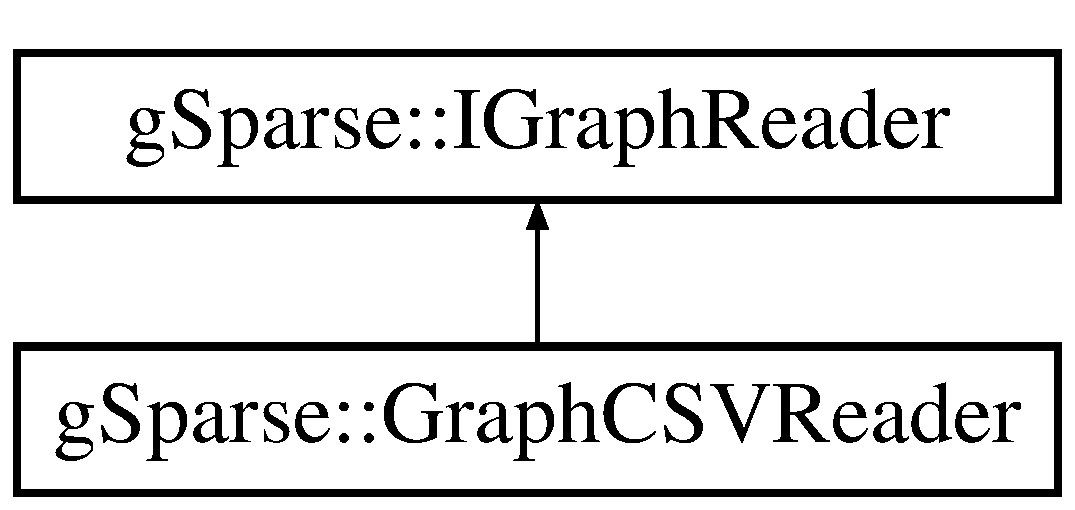
\includegraphics[height=2.000000cm]{classg_sparse_1_1_graph_c_s_v_reader}
\end{center}
\end{figure}
\subsection*{Public Member Functions}
\begin{DoxyCompactItemize}
\item 
\mbox{\Hypertarget{classg_sparse_1_1_graph_c_s_v_reader_ac0609b1dbd62f3425d6108caeeafcea7}\label{classg_sparse_1_1_graph_c_s_v_reader_ac0609b1dbd62f3425d6108caeeafcea7}} 
\mbox{\hyperlink{classg_sparse_1_1_graph_c_s_v_reader_ac0609b1dbd62f3425d6108caeeafcea7}{Graph\+C\+S\+V\+Reader}} (const \mbox{\hyperlink{classg_sparse_1_1_graph_c_s_v_reader}{Graph\+C\+S\+V\+Reader}} \&csv\+Reader) noexcept
\begin{DoxyCompactList}\small\item\em A copy Constructor. \end{DoxyCompactList}\item 
\mbox{\Hypertarget{classg_sparse_1_1_graph_c_s_v_reader_a9736ef3836d11b7d4cd095b0613410d5}\label{classg_sparse_1_1_graph_c_s_v_reader_a9736ef3836d11b7d4cd095b0613410d5}} 
\mbox{\hyperlink{classg_sparse_1_1_graph_c_s_v_reader}{Graph\+C\+S\+V\+Reader}} \& \mbox{\hyperlink{classg_sparse_1_1_graph_c_s_v_reader_a9736ef3836d11b7d4cd095b0613410d5}{operator=}} (const \mbox{\hyperlink{classg_sparse_1_1_graph_c_s_v_reader}{Graph\+C\+S\+V\+Reader}} \&csv\+Reader) noexcept
\begin{DoxyCompactList}\small\item\em A = operator overloaded. \end{DoxyCompactList}\item 
\mbox{\hyperlink{classg_sparse_1_1_graph_c_s_v_reader_a5c95cc40faadeaa36766b05b3b4079d0}{Graph\+C\+S\+V\+Reader}} (const std\+::string \&Edge\+File\+Name, const std\+::string \&Weight\+File\+Name=\char`\"{}None\char`\"{}, const std\+::string \&delimeter=\char`\"{},\char`\"{})
\begin{DoxyCompactList}\small\item\em Constructor. \end{DoxyCompactList}\item 
virtual void \mbox{\hyperlink{classg_sparse_1_1_graph_c_s_v_reader_a01218efe45c694d0b721e737e9c53365}{Read}} (g\+Sparse\+::\+Edge\+Matrix \&Edges, g\+Sparse\+::\+Precision\+Row\+Matrix \&Weights)
\begin{DoxyCompactList}\small\item\em Read graph data from a C\+SV file specified in the constructor. \end{DoxyCompactList}\item 
\mbox{\Hypertarget{classg_sparse_1_1_graph_c_s_v_reader_a698d7bab55ff0857f264b3a6cc79d02f}\label{classg_sparse_1_1_graph_c_s_v_reader_a698d7bab55ff0857f264b3a6cc79d02f}} 
\mbox{\hyperlink{classg_sparse_1_1_graph_c_s_v_reader_a698d7bab55ff0857f264b3a6cc79d02f}{$\sim$\+Graph\+C\+S\+V\+Reader}} ()=default
\begin{DoxyCompactList}\small\item\em Default destructor. \end{DoxyCompactList}\end{DoxyCompactItemize}


\subsection{Detailed Description}
A Graph C\+SV Data Reader. 

This class reads Graph Edge and List C\+SV files and transform them into Eigen Matrix. Node index starts from zero. Weight data type is g\+Sparse\+::\+P\+R\+E\+C\+I\+S\+I\+ON type defined in \mbox{\hyperlink{_config_8hpp_source}{Config.\+hpp}} 

\subsection{Constructor \& Destructor Documentation}
\mbox{\Hypertarget{classg_sparse_1_1_graph_c_s_v_reader_a5c95cc40faadeaa36766b05b3b4079d0}\label{classg_sparse_1_1_graph_c_s_v_reader_a5c95cc40faadeaa36766b05b3b4079d0}} 
\index{g\+Sparse\+::\+Graph\+C\+S\+V\+Reader@{g\+Sparse\+::\+Graph\+C\+S\+V\+Reader}!Graph\+C\+S\+V\+Reader@{Graph\+C\+S\+V\+Reader}}
\index{Graph\+C\+S\+V\+Reader@{Graph\+C\+S\+V\+Reader}!g\+Sparse\+::\+Graph\+C\+S\+V\+Reader@{g\+Sparse\+::\+Graph\+C\+S\+V\+Reader}}
\subsubsection{\texorpdfstring{Graph\+C\+S\+V\+Reader()}{GraphCSVReader()}}
{\footnotesize\ttfamily g\+Sparse\+::\+Graph\+C\+S\+V\+Reader\+::\+Graph\+C\+S\+V\+Reader (\begin{DoxyParamCaption}\item[{const std\+::string \&}]{Edge\+File\+Name,  }\item[{const std\+::string \&}]{Weight\+File\+Name = {\ttfamily \char`\"{}None\char`\"{}},  }\item[{const std\+::string \&}]{delimeter = {\ttfamily \char`\"{},\char`\"{}} }\end{DoxyParamCaption})\hspace{0.3cm}{\ttfamily [inline]}}



Constructor. 


\begin{DoxyParams}{Parameters}
{\em Edge\+File\+Name} & A filename pointing to a C\+SV file that contains Edge list. \\
\hline
{\em Weight\+File\+Name} & A filename pointing to a C\+SV file that contains weight list. Default is \char`\"{}\+None\char`\"{}\+: all weights equal to one. \\
\hline
{\em delimeter} & A delimeter of the C\+SV file. Default is a comma (,). \\
\hline
\end{DoxyParams}


\subsection{Member Function Documentation}
\mbox{\Hypertarget{classg_sparse_1_1_graph_c_s_v_reader_a01218efe45c694d0b721e737e9c53365}\label{classg_sparse_1_1_graph_c_s_v_reader_a01218efe45c694d0b721e737e9c53365}} 
\index{g\+Sparse\+::\+Graph\+C\+S\+V\+Reader@{g\+Sparse\+::\+Graph\+C\+S\+V\+Reader}!Read@{Read}}
\index{Read@{Read}!g\+Sparse\+::\+Graph\+C\+S\+V\+Reader@{g\+Sparse\+::\+Graph\+C\+S\+V\+Reader}}
\subsubsection{\texorpdfstring{Read()}{Read()}}
{\footnotesize\ttfamily virtual void g\+Sparse\+::\+Graph\+C\+S\+V\+Reader\+::\+Read (\begin{DoxyParamCaption}\item[{g\+Sparse\+::\+Edge\+Matrix \&}]{Edges,  }\item[{g\+Sparse\+::\+Precision\+Row\+Matrix \&}]{Weights }\end{DoxyParamCaption})\hspace{0.3cm}{\ttfamily [inline]}, {\ttfamily [virtual]}}



Read graph data from a C\+SV file specified in the constructor. 


\begin{DoxyParams}{Parameters}
{\em Edges} & An Eigen Matrix to receive the Edge list. \\
\hline
{\em Weights} & An Eigen Matrix to receive the Weight list. \\
\hline
\end{DoxyParams}


Implements \mbox{\hyperlink{classg_sparse_1_1_i_graph_reader_a42885505f5bdb8136b0d5b386925d1c7}{g\+Sparse\+::\+I\+Graph\+Reader}}.



The documentation for this class was generated from the following file\+:\begin{DoxyCompactItemize}
\item 
/\+Users/\+Bomb/\+Documents/\+Project/g\+Sparse/include/g\+Sparse/Graph\+C\+S\+V\+Reader.\+hpp\end{DoxyCompactItemize}

\hypertarget{classg_sparse_1_1_graph_c_s_v_writer}{}\section{g\+Sparse\+:\+:Graph\+C\+S\+V\+Writer Class Reference}
\label{classg_sparse_1_1_graph_c_s_v_writer}\index{g\+Sparse\+::\+Graph\+C\+S\+V\+Writer@{g\+Sparse\+::\+Graph\+C\+S\+V\+Writer}}


A Graph C\+SV Data Writer.  




{\ttfamily \#include $<$Graph\+C\+S\+V\+Writer.\+hpp$>$}

Inheritance diagram for g\+Sparse\+:\+:Graph\+C\+S\+V\+Writer\+:\begin{figure}[H]
\begin{center}
\leavevmode
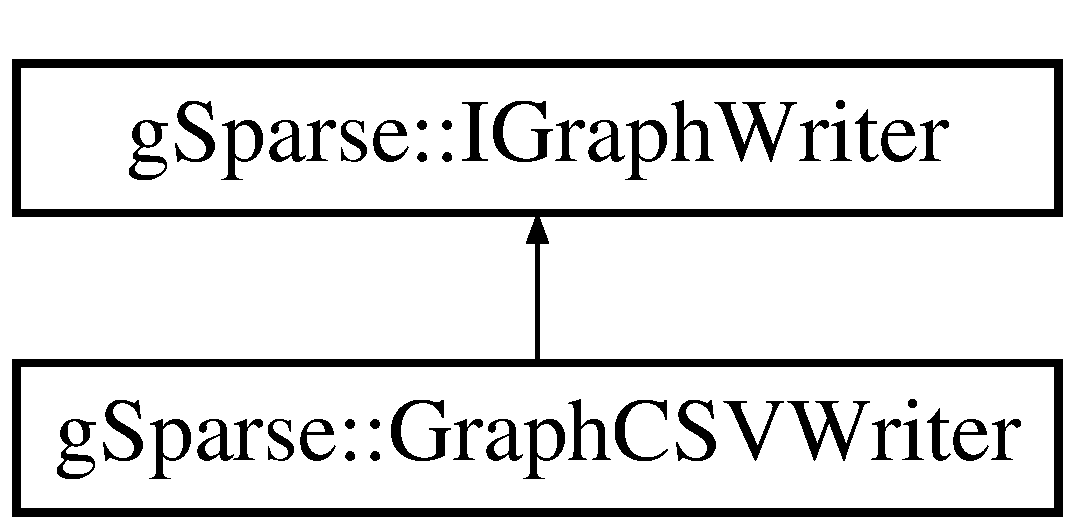
\includegraphics[height=2.000000cm]{classg_sparse_1_1_graph_c_s_v_writer}
\end{center}
\end{figure}
\subsection*{Public Member Functions}
\begin{DoxyCompactItemize}
\item 
\mbox{\Hypertarget{classg_sparse_1_1_graph_c_s_v_writer_a72f27412732680150f6706f456db93c4}\label{classg_sparse_1_1_graph_c_s_v_writer_a72f27412732680150f6706f456db93c4}} 
\mbox{\hyperlink{classg_sparse_1_1_graph_c_s_v_writer_a72f27412732680150f6706f456db93c4}{Graph\+C\+S\+V\+Writer}} (const \mbox{\hyperlink{classg_sparse_1_1_graph_c_s_v_writer}{Graph\+C\+S\+V\+Writer}} \&csv\+Reader) noexcept
\begin{DoxyCompactList}\small\item\em A copy Constructor. \end{DoxyCompactList}\item 
\mbox{\Hypertarget{classg_sparse_1_1_graph_c_s_v_writer_ab0b254d0861f2bb0edc789e6f080a912}\label{classg_sparse_1_1_graph_c_s_v_writer_ab0b254d0861f2bb0edc789e6f080a912}} 
\mbox{\hyperlink{classg_sparse_1_1_graph_c_s_v_writer}{Graph\+C\+S\+V\+Writer}} \& \mbox{\hyperlink{classg_sparse_1_1_graph_c_s_v_writer_ab0b254d0861f2bb0edc789e6f080a912}{operator=}} (const \mbox{\hyperlink{classg_sparse_1_1_graph_c_s_v_writer}{Graph\+C\+S\+V\+Writer}} \&csv\+Reader) noexcept
\begin{DoxyCompactList}\small\item\em A = operator overloaded. \end{DoxyCompactList}\item 
\mbox{\hyperlink{classg_sparse_1_1_graph_c_s_v_writer_aa89f61ce6e6affcbc418f892f0110de9}{Graph\+C\+S\+V\+Writer}} (const std\+::string \&Edge\+File\+Name, const std\+::string \&Weight\+File\+Name=\char`\"{}None\char`\"{}, std\+::string delimeter=\char`\"{},\char`\"{})
\begin{DoxyCompactList}\small\item\em Constructor. \end{DoxyCompactList}\item 
virtual void \mbox{\hyperlink{classg_sparse_1_1_graph_c_s_v_writer_a588c4bf47ee70bb72079ac7d6f843c2d}{Write}} (const g\+Sparse\+::\+Graph \&graph)
\begin{DoxyCompactList}\small\item\em Write graph data to a C\+SV file specified in the constructor. \end{DoxyCompactList}\item 
virtual void \mbox{\hyperlink{classg_sparse_1_1_graph_c_s_v_writer_a83598d104e12327bf819928239e18ca3}{Write}} (const g\+Sparse\+::\+Edge\+Matrix \&Edges)
\begin{DoxyCompactList}\small\item\em Write graph data to a C\+SV file specified in the constructor. \end{DoxyCompactList}\item 
virtual void \mbox{\hyperlink{classg_sparse_1_1_graph_c_s_v_writer_a66e9fe4e8887abca81d6d0090b217950}{Write}} (const g\+Sparse\+::\+Edge\+Matrix \&Edges, const g\+Sparse\+::\+Precision\+Row\+Matrix \&Weights)
\begin{DoxyCompactList}\small\item\em Write graph data to a C\+SV file specified in the constructor. \end{DoxyCompactList}\end{DoxyCompactItemize}


\subsection{Detailed Description}
A Graph C\+SV Data Writer. 

This class writes Graph Edge and List C\+SV files based on given input Node index starts from zero. Weight data type is g\+Sparse\+::\+P\+R\+E\+C\+I\+S\+I\+ON type defined in \mbox{\hyperlink{_config_8hpp_source}{Config.\+hpp}} 

\subsection{Constructor \& Destructor Documentation}
\mbox{\Hypertarget{classg_sparse_1_1_graph_c_s_v_writer_aa89f61ce6e6affcbc418f892f0110de9}\label{classg_sparse_1_1_graph_c_s_v_writer_aa89f61ce6e6affcbc418f892f0110de9}} 
\index{g\+Sparse\+::\+Graph\+C\+S\+V\+Writer@{g\+Sparse\+::\+Graph\+C\+S\+V\+Writer}!Graph\+C\+S\+V\+Writer@{Graph\+C\+S\+V\+Writer}}
\index{Graph\+C\+S\+V\+Writer@{Graph\+C\+S\+V\+Writer}!g\+Sparse\+::\+Graph\+C\+S\+V\+Writer@{g\+Sparse\+::\+Graph\+C\+S\+V\+Writer}}
\subsubsection{\texorpdfstring{Graph\+C\+S\+V\+Writer()}{GraphCSVWriter()}}
{\footnotesize\ttfamily g\+Sparse\+::\+Graph\+C\+S\+V\+Writer\+::\+Graph\+C\+S\+V\+Writer (\begin{DoxyParamCaption}\item[{const std\+::string \&}]{Edge\+File\+Name,  }\item[{const std\+::string \&}]{Weight\+File\+Name = {\ttfamily \char`\"{}None\char`\"{}},  }\item[{std\+::string}]{delimeter = {\ttfamily \char`\"{},\char`\"{}} }\end{DoxyParamCaption})\hspace{0.3cm}{\ttfamily [inline]}}



Constructor. 


\begin{DoxyParams}{Parameters}
{\em Edge\+File\+Name} & A filename pointing to a C\+SV file that contains Edge list. \\
\hline
{\em Weight\+File\+Name} & A filename pointing to a C\+SV file that contains weight list. Default is \char`\"{}\+None\char`\"{}\+: all weights equal to one. \\
\hline
{\em delimeter} & A delimeter of the C\+SV file. Default is a comma (,). \\
\hline
\end{DoxyParams}


\subsection{Member Function Documentation}
\mbox{\Hypertarget{classg_sparse_1_1_graph_c_s_v_writer_a588c4bf47ee70bb72079ac7d6f843c2d}\label{classg_sparse_1_1_graph_c_s_v_writer_a588c4bf47ee70bb72079ac7d6f843c2d}} 
\index{g\+Sparse\+::\+Graph\+C\+S\+V\+Writer@{g\+Sparse\+::\+Graph\+C\+S\+V\+Writer}!Write@{Write}}
\index{Write@{Write}!g\+Sparse\+::\+Graph\+C\+S\+V\+Writer@{g\+Sparse\+::\+Graph\+C\+S\+V\+Writer}}
\subsubsection{\texorpdfstring{Write()}{Write()}\hspace{0.1cm}{\footnotesize\ttfamily [1/3]}}
{\footnotesize\ttfamily virtual void g\+Sparse\+::\+Graph\+C\+S\+V\+Writer\+::\+Write (\begin{DoxyParamCaption}\item[{const g\+Sparse\+::\+Graph \&}]{graph }\end{DoxyParamCaption})\hspace{0.3cm}{\ttfamily [inline]}, {\ttfamily [virtual]}}



Write graph data to a C\+SV file specified in the constructor. 


\begin{DoxyParams}{Parameters}
{\em graph} & A graph object \\
\hline
\end{DoxyParams}


Implements \mbox{\hyperlink{classg_sparse_1_1_i_graph_writer_a24a0956558888343c5e56a3c39b138af}{g\+Sparse\+::\+I\+Graph\+Writer}}.

\mbox{\Hypertarget{classg_sparse_1_1_graph_c_s_v_writer_a83598d104e12327bf819928239e18ca3}\label{classg_sparse_1_1_graph_c_s_v_writer_a83598d104e12327bf819928239e18ca3}} 
\index{g\+Sparse\+::\+Graph\+C\+S\+V\+Writer@{g\+Sparse\+::\+Graph\+C\+S\+V\+Writer}!Write@{Write}}
\index{Write@{Write}!g\+Sparse\+::\+Graph\+C\+S\+V\+Writer@{g\+Sparse\+::\+Graph\+C\+S\+V\+Writer}}
\subsubsection{\texorpdfstring{Write()}{Write()}\hspace{0.1cm}{\footnotesize\ttfamily [2/3]}}
{\footnotesize\ttfamily virtual void g\+Sparse\+::\+Graph\+C\+S\+V\+Writer\+::\+Write (\begin{DoxyParamCaption}\item[{const g\+Sparse\+::\+Edge\+Matrix \&}]{Edges }\end{DoxyParamCaption})\hspace{0.3cm}{\ttfamily [inline]}, {\ttfamily [virtual]}}



Write graph data to a C\+SV file specified in the constructor. 


\begin{DoxyParams}{Parameters}
{\em Edges} & An edge list to be written to a C\+SV file \\
\hline
\end{DoxyParams}


Implements \mbox{\hyperlink{classg_sparse_1_1_i_graph_writer_aa778df52e1595439d724fc873a8dfb52}{g\+Sparse\+::\+I\+Graph\+Writer}}.

\mbox{\Hypertarget{classg_sparse_1_1_graph_c_s_v_writer_a66e9fe4e8887abca81d6d0090b217950}\label{classg_sparse_1_1_graph_c_s_v_writer_a66e9fe4e8887abca81d6d0090b217950}} 
\index{g\+Sparse\+::\+Graph\+C\+S\+V\+Writer@{g\+Sparse\+::\+Graph\+C\+S\+V\+Writer}!Write@{Write}}
\index{Write@{Write}!g\+Sparse\+::\+Graph\+C\+S\+V\+Writer@{g\+Sparse\+::\+Graph\+C\+S\+V\+Writer}}
\subsubsection{\texorpdfstring{Write()}{Write()}\hspace{0.1cm}{\footnotesize\ttfamily [3/3]}}
{\footnotesize\ttfamily virtual void g\+Sparse\+::\+Graph\+C\+S\+V\+Writer\+::\+Write (\begin{DoxyParamCaption}\item[{const g\+Sparse\+::\+Edge\+Matrix \&}]{Edges,  }\item[{const g\+Sparse\+::\+Precision\+Row\+Matrix \&}]{Weights }\end{DoxyParamCaption})\hspace{0.3cm}{\ttfamily [inline]}, {\ttfamily [virtual]}}



Write graph data to a C\+SV file specified in the constructor. 


\begin{DoxyParams}{Parameters}
{\em Edges} & An edge list to be written to a C\+SV file \\
\hline
{\em Weights} & A weight list to be written to a C\+SV file \\
\hline
\end{DoxyParams}


Implements \mbox{\hyperlink{classg_sparse_1_1_i_graph_writer_ae2c720f3e37629da40fdc5d0e4fe2dd2}{g\+Sparse\+::\+I\+Graph\+Writer}}.



The documentation for this class was generated from the following file\+:\begin{DoxyCompactItemize}
\item 
/\+Users/\+Bomb/\+Documents/\+Project/g\+Sparse/include/g\+Sparse/Graph\+C\+S\+V\+Writer.\+hpp\end{DoxyCompactItemize}

\hypertarget{classg_sparse_1_1_i_effective_resistance}{}\section{g\+Sparse\+:\+:I\+Effective\+Resistance Class Reference}
\label{classg_sparse_1_1_i_effective_resistance}\index{g\+Sparse\+::\+I\+Effective\+Resistance@{g\+Sparse\+::\+I\+Effective\+Resistance}}


An interface class for Effective Resistance Calculator.  




{\ttfamily \#include $<$Effective\+Resistance.\+hpp$>$}

Inheritance diagram for g\+Sparse\+:\+:I\+Effective\+Resistance\+:\begin{figure}[H]
\begin{center}
\leavevmode
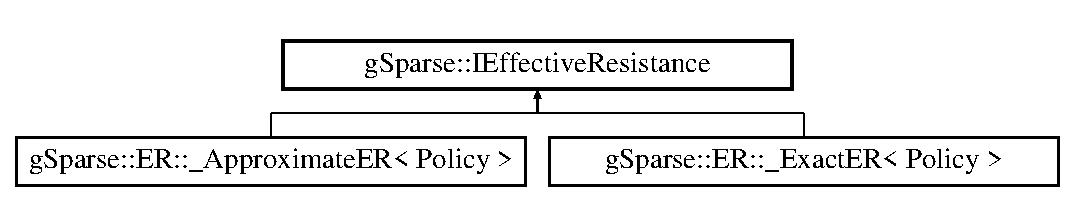
\includegraphics[height=2.000000cm]{classg_sparse_1_1_i_effective_resistance}
\end{center}
\end{figure}
\subsection*{Public Member Functions}
\begin{DoxyCompactItemize}
\item 
\mbox{\Hypertarget{classg_sparse_1_1_i_effective_resistance_aa1f38b056757c2b25a22a6eaa87aa50f}\label{classg_sparse_1_1_i_effective_resistance_aa1f38b056757c2b25a22a6eaa87aa50f}} 
virtual g\+Sparse\+::\+C\+O\+M\+P\+U\+T\+E\+\_\+\+I\+N\+FO \mbox{\hyperlink{classg_sparse_1_1_i_effective_resistance_aa1f38b056757c2b25a22a6eaa87aa50f}{Calculate\+ER}} (g\+Sparse\+::\+Precision\+Row\+Matrix \&, const g\+Sparse\+::\+Graph \&)=0
\begin{DoxyCompactList}\small\item\em A pure virtual member to computer sparsifier weight. \end{DoxyCompactList}\end{DoxyCompactItemize}


\subsection{Detailed Description}
An interface class for Effective Resistance Calculator. 

This class defines an interface for g\+Sparse\textquotesingle{}s Effective\+Resistance 

The documentation for this class was generated from the following file\+:\begin{DoxyCompactItemize}
\item 
/\+Users/\+Bomb/\+Documents/\+Project/g\+Sparse/include/g\+Sparse/\+Interface/Effective\+Resistance.\+hpp\end{DoxyCompactItemize}

\hypertarget{classg_sparse_1_1_i_graph}{}\section{g\+Sparse\+:\+:I\+Graph Class Reference}
\label{classg_sparse_1_1_i_graph}\index{g\+Sparse\+::\+I\+Graph@{g\+Sparse\+::\+I\+Graph}}


An interface class for Graph object.  




{\ttfamily \#include $<$Graph.\+hpp$>$}

Inheritance diagram for g\+Sparse\+:\+:I\+Graph\+:\begin{figure}[H]
\begin{center}
\leavevmode
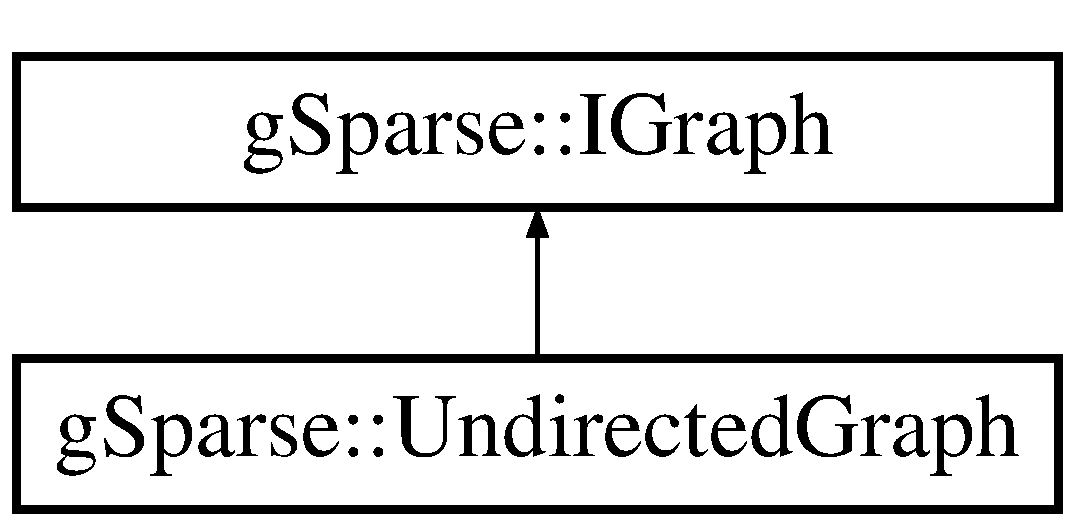
\includegraphics[height=2.000000cm]{classg_sparse_1_1_i_graph}
\end{center}
\end{figure}
\subsection*{Public Member Functions}
\begin{DoxyCompactItemize}
\item 
\mbox{\Hypertarget{classg_sparse_1_1_i_graph_af154d74864aba40ebb121d921090682e}\label{classg_sparse_1_1_i_graph_af154d74864aba40ebb121d921090682e}} 
virtual const g\+Sparse\+::\+Sparse\+Precision\+Matrix \& \mbox{\hyperlink{classg_sparse_1_1_i_graph_af154d74864aba40ebb121d921090682e}{Get\+Adjacent\+Matrix}} () const =0
\begin{DoxyCompactList}\small\item\em Pure virtual function to get Graph Adjacency Matrix. \end{DoxyCompactList}\item 
\mbox{\Hypertarget{classg_sparse_1_1_i_graph_a2c748303c9f5da63fa5da90a1110633f}\label{classg_sparse_1_1_i_graph_a2c748303c9f5da63fa5da90a1110633f}} 
virtual const g\+Sparse\+::\+Sparse\+Precision\+Matrix \& \mbox{\hyperlink{classg_sparse_1_1_i_graph_a2c748303c9f5da63fa5da90a1110633f}{Get\+Incident\+Matrix}} () const =0
\begin{DoxyCompactList}\small\item\em Pure virtual function to get Graph Incident Matrix. \end{DoxyCompactList}\item 
\mbox{\Hypertarget{classg_sparse_1_1_i_graph_a24465b20eba67a564b620b21f174da89}\label{classg_sparse_1_1_i_graph_a24465b20eba67a564b620b21f174da89}} 
virtual const g\+Sparse\+::\+Sparse\+Precision\+Matrix \& \mbox{\hyperlink{classg_sparse_1_1_i_graph_a24465b20eba67a564b620b21f174da89}{Get\+Degree\+Matrix}} () const =0
\begin{DoxyCompactList}\small\item\em Pure virtual function to get Graph Degree Matrix. \end{DoxyCompactList}\item 
\mbox{\Hypertarget{classg_sparse_1_1_i_graph_a861e57ebfe47eb54236e82f8651f398c}\label{classg_sparse_1_1_i_graph_a861e57ebfe47eb54236e82f8651f398c}} 
virtual const g\+Sparse\+::\+Sparse\+Precision\+Matrix \& \mbox{\hyperlink{classg_sparse_1_1_i_graph_a861e57ebfe47eb54236e82f8651f398c}{Get\+Laplacian\+Matrix}} () const =0
\begin{DoxyCompactList}\small\item\em Pure virtual function to get Graph Laplacian Matrix. \end{DoxyCompactList}\item 
\mbox{\Hypertarget{classg_sparse_1_1_i_graph_aef60a9eb32de1ceb2a62313a54609ac4}\label{classg_sparse_1_1_i_graph_aef60a9eb32de1ceb2a62313a54609ac4}} 
virtual const g\+Sparse\+::\+Sparse\+Precision\+Matrix \& \mbox{\hyperlink{classg_sparse_1_1_i_graph_aef60a9eb32de1ceb2a62313a54609ac4}{Get\+Weight\+Matrix}} () const =0
\begin{DoxyCompactList}\small\item\em Pure virtual function to get Graph Weight Matrix. \end{DoxyCompactList}\item 
\mbox{\Hypertarget{classg_sparse_1_1_i_graph_ad7bc73bd80951ccb15f391c02a1def23}\label{classg_sparse_1_1_i_graph_ad7bc73bd80951ccb15f391c02a1def23}} 
virtual const g\+Sparse\+::\+Edge\+Matrix \& \mbox{\hyperlink{classg_sparse_1_1_i_graph_ad7bc73bd80951ccb15f391c02a1def23}{Get\+Edge\+List}} () const =0
\begin{DoxyCompactList}\small\item\em Pure virtual function to get Graph Edge List Matrix. \end{DoxyCompactList}\item 
\mbox{\Hypertarget{classg_sparse_1_1_i_graph_a4230acbf3a86759fe6a5e19c3293adc7}\label{classg_sparse_1_1_i_graph_a4230acbf3a86759fe6a5e19c3293adc7}} 
virtual const g\+Sparse\+::\+Precision\+Row\+Matrix \& \mbox{\hyperlink{classg_sparse_1_1_i_graph_a4230acbf3a86759fe6a5e19c3293adc7}{Get\+Weight\+List}} () const =0
\begin{DoxyCompactList}\small\item\em Pure virtual function to get Graph Weight List Matrix. \end{DoxyCompactList}\item 
\mbox{\Hypertarget{classg_sparse_1_1_i_graph_a0dc8f4d2283a175876cf8e56a7979e78}\label{classg_sparse_1_1_i_graph_a0dc8f4d2283a175876cf8e56a7979e78}} 
virtual std\+::size\+\_\+t \mbox{\hyperlink{classg_sparse_1_1_i_graph_a0dc8f4d2283a175876cf8e56a7979e78}{Get\+Edge\+Count}} () const =0
\begin{DoxyCompactList}\small\item\em Pure virtual function to get number of edges in the graph. \end{DoxyCompactList}\item 
\mbox{\Hypertarget{classg_sparse_1_1_i_graph_a810e7c5a7e011f516b4a8ae56fe8ce3b}\label{classg_sparse_1_1_i_graph_a810e7c5a7e011f516b4a8ae56fe8ce3b}} 
virtual std\+::size\+\_\+t \mbox{\hyperlink{classg_sparse_1_1_i_graph_a810e7c5a7e011f516b4a8ae56fe8ce3b}{Get\+Node\+Count}} () const =0
\begin{DoxyCompactList}\small\item\em Pure virtual function to get number of nodes in the graph. \end{DoxyCompactList}\end{DoxyCompactItemize}
\subsection*{Protected Member Functions}
\begin{DoxyCompactItemize}
\item 
\mbox{\Hypertarget{classg_sparse_1_1_i_graph_a49f79b460e4166da28dd0f188bd0e34e}\label{classg_sparse_1_1_i_graph_a49f79b460e4166da28dd0f188bd0e34e}} 
\mbox{\hyperlink{classg_sparse_1_1_i_graph_a49f79b460e4166da28dd0f188bd0e34e}{I\+Graph}} ()=default
\begin{DoxyCompactList}\small\item\em Protected default constructor. \end{DoxyCompactList}\end{DoxyCompactItemize}


\subsection{Detailed Description}
An interface class for Graph object. 

This class defines an interface for g\+Sparse\textquotesingle{}s Graph primitives. 

The documentation for this class was generated from the following file\+:\begin{DoxyCompactItemize}
\item 
/\+Users/\+Bomb/\+Documents/\+Project/g\+Sparse/include/g\+Sparse/\+Interface/Graph.\+hpp\end{DoxyCompactItemize}

\hypertarget{classg_sparse_1_1_i_graph_reader}{}\section{g\+Sparse\+:\+:I\+Graph\+Reader Class Reference}
\label{classg_sparse_1_1_i_graph_reader}\index{g\+Sparse\+::\+I\+Graph\+Reader@{g\+Sparse\+::\+I\+Graph\+Reader}}


An interface class for Graph Input.  




{\ttfamily \#include $<$Graph\+Reader.\+hpp$>$}

Inheritance diagram for g\+Sparse\+:\+:I\+Graph\+Reader\+:\begin{figure}[H]
\begin{center}
\leavevmode
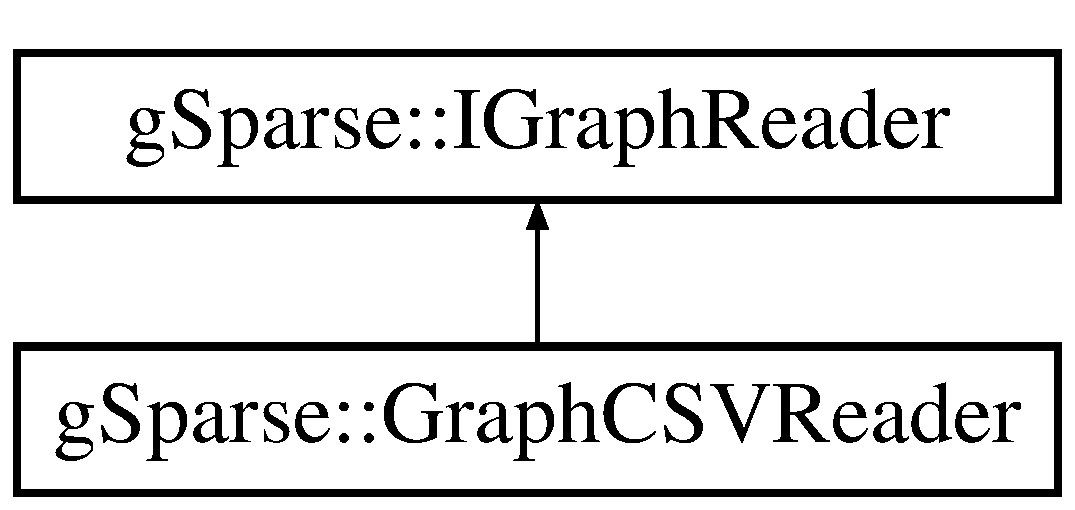
\includegraphics[height=2.000000cm]{classg_sparse_1_1_i_graph_reader}
\end{center}
\end{figure}
\subsection*{Public Member Functions}
\begin{DoxyCompactItemize}
\item 
\mbox{\Hypertarget{classg_sparse_1_1_i_graph_reader_adc903c78e5b76aebca391b2b07ec81d7}\label{classg_sparse_1_1_i_graph_reader_adc903c78e5b76aebca391b2b07ec81d7}} 
\mbox{\hyperlink{classg_sparse_1_1_i_graph_reader_adc903c78e5b76aebca391b2b07ec81d7}{I\+Graph\+Reader}} ()=default
\begin{DoxyCompactList}\small\item\em Default Constructor for \mbox{\hyperlink{classg_sparse_1_1_i_graph_reader}{I\+Graph\+Reader}}. \end{DoxyCompactList}\item 
virtual void \mbox{\hyperlink{classg_sparse_1_1_i_graph_reader_a42885505f5bdb8136b0d5b386925d1c7}{Read}} (g\+Sparse\+::\+Edge\+Matrix \&Edges, g\+Sparse\+::\+Precision\+Row\+Matrix \&Weights)=0
\begin{DoxyCompactList}\small\item\em A pure virtual member to read Graph Data by passing two reference for input. \end{DoxyCompactList}\item 
\mbox{\Hypertarget{classg_sparse_1_1_i_graph_reader_a03a04fad2268a001b23bcafb5391b894}\label{classg_sparse_1_1_i_graph_reader_a03a04fad2268a001b23bcafb5391b894}} 
virtual \mbox{\hyperlink{classg_sparse_1_1_i_graph_reader_a03a04fad2268a001b23bcafb5391b894}{$\sim$\+I\+Graph\+Reader}} ()=default
\begin{DoxyCompactList}\small\item\em Default virtual destructor. \end{DoxyCompactList}\end{DoxyCompactItemize}


\subsection{Detailed Description}
An interface class for Graph Input. 

This class defines an interface for g\+Sparse\textquotesingle{}s graph reading functionality. New input source should derive from this class. 

\subsection{Member Function Documentation}
\mbox{\Hypertarget{classg_sparse_1_1_i_graph_reader_a42885505f5bdb8136b0d5b386925d1c7}\label{classg_sparse_1_1_i_graph_reader_a42885505f5bdb8136b0d5b386925d1c7}} 
\index{g\+Sparse\+::\+I\+Graph\+Reader@{g\+Sparse\+::\+I\+Graph\+Reader}!Read@{Read}}
\index{Read@{Read}!g\+Sparse\+::\+I\+Graph\+Reader@{g\+Sparse\+::\+I\+Graph\+Reader}}
\subsubsection{\texorpdfstring{Read()}{Read()}}
{\footnotesize\ttfamily virtual void g\+Sparse\+::\+I\+Graph\+Reader\+::\+Read (\begin{DoxyParamCaption}\item[{g\+Sparse\+::\+Edge\+Matrix \&}]{Edges,  }\item[{g\+Sparse\+::\+Precision\+Row\+Matrix \&}]{Weights }\end{DoxyParamCaption})\hspace{0.3cm}{\ttfamily [pure virtual]}}



A pure virtual member to read Graph Data by passing two reference for input. 


\begin{DoxyParams}{Parameters}
{\em Edges} & An Eigen Matrix to receive the Edge list. \\
\hline
{\em Weights} & An Eigen Matrix to receive the Weight list associated to the Edge list. \\
\hline
\end{DoxyParams}


Implemented in \mbox{\hyperlink{classg_sparse_1_1_graph_c_s_v_reader_a01218efe45c694d0b721e737e9c53365}{g\+Sparse\+::\+Graph\+C\+S\+V\+Reader}}.



The documentation for this class was generated from the following file\+:\begin{DoxyCompactItemize}
\item 
/\+Users/\+Bomb/\+Documents/\+Project/g\+Sparse/include/g\+Sparse/\+Interface/Graph\+Reader.\+hpp\end{DoxyCompactItemize}

\hypertarget{classg_sparse_1_1_i_graph_writer}{}\section{g\+Sparse\+:\+:I\+Graph\+Writer Class Reference}
\label{classg_sparse_1_1_i_graph_writer}\index{g\+Sparse\+::\+I\+Graph\+Writer@{g\+Sparse\+::\+I\+Graph\+Writer}}


An interface class for Graph Output.  




{\ttfamily \#include $<$Graph\+Writer.\+hpp$>$}

Inheritance diagram for g\+Sparse\+:\+:I\+Graph\+Writer\+:\begin{figure}[H]
\begin{center}
\leavevmode
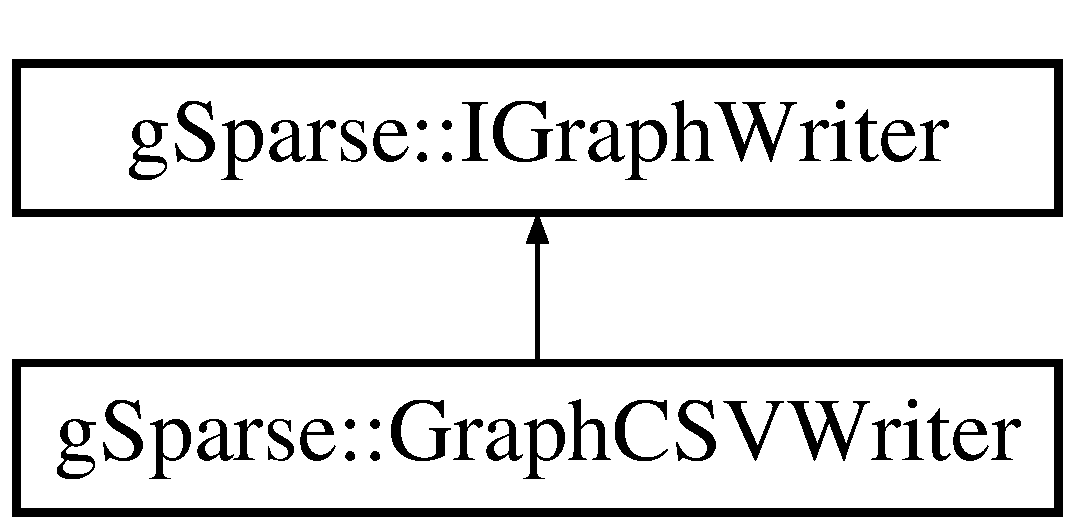
\includegraphics[height=2.000000cm]{classg_sparse_1_1_i_graph_writer}
\end{center}
\end{figure}
\subsection*{Public Member Functions}
\begin{DoxyCompactItemize}
\item 
\mbox{\Hypertarget{classg_sparse_1_1_i_graph_writer_a05a22eb501d282bc3617e034ac6ce2af}\label{classg_sparse_1_1_i_graph_writer_a05a22eb501d282bc3617e034ac6ce2af}} 
\mbox{\hyperlink{classg_sparse_1_1_i_graph_writer_a05a22eb501d282bc3617e034ac6ce2af}{I\+Graph\+Writer}} ()=default
\begin{DoxyCompactList}\small\item\em Default Constructor for \mbox{\hyperlink{classg_sparse_1_1_i_graph_writer}{I\+Graph\+Writer}}. \end{DoxyCompactList}\item 
virtual void \mbox{\hyperlink{classg_sparse_1_1_i_graph_writer_a24a0956558888343c5e56a3c39b138af}{Write}} (const g\+Sparse\+::\+Graph \&graph)=0
\begin{DoxyCompactList}\small\item\em A pure virtual member write Graph Data by passing an \mbox{\hyperlink{classg_sparse_1_1_i_graph}{I\+Graph}} object. \end{DoxyCompactList}\item 
virtual void \mbox{\hyperlink{classg_sparse_1_1_i_graph_writer_aa778df52e1595439d724fc873a8dfb52}{Write}} (const g\+Sparse\+::\+Edge\+Matrix \&Edges)=0
\begin{DoxyCompactList}\small\item\em A pure virtual member write Graph Data by passing Edge List. \end{DoxyCompactList}\item 
virtual void \mbox{\hyperlink{classg_sparse_1_1_i_graph_writer_ae2c720f3e37629da40fdc5d0e4fe2dd2}{Write}} (const g\+Sparse\+::\+Edge\+Matrix \&Edges, const g\+Sparse\+::\+Precision\+Row\+Matrix \&Weights)=0
\begin{DoxyCompactList}\small\item\em A pure virtual member write read Graph Data by passing an Edge and a Weight Lists. \end{DoxyCompactList}\item 
\mbox{\Hypertarget{classg_sparse_1_1_i_graph_writer_a7c29459ba96e82fec35b1a71a8d79e05}\label{classg_sparse_1_1_i_graph_writer_a7c29459ba96e82fec35b1a71a8d79e05}} 
virtual \mbox{\hyperlink{classg_sparse_1_1_i_graph_writer_a7c29459ba96e82fec35b1a71a8d79e05}{$\sim$\+I\+Graph\+Writer}} ()=default
\begin{DoxyCompactList}\small\item\em Default Constructor for \mbox{\hyperlink{classg_sparse_1_1_i_graph_writer}{I\+Graph\+Writer}}. \end{DoxyCompactList}\end{DoxyCompactItemize}


\subsection{Detailed Description}
An interface class for Graph Output. 

This class defines an interface for g\+Sparse\textquotesingle{}s graph writing functionality. New output source should derive this function. 

\subsection{Member Function Documentation}
\mbox{\Hypertarget{classg_sparse_1_1_i_graph_writer_a24a0956558888343c5e56a3c39b138af}\label{classg_sparse_1_1_i_graph_writer_a24a0956558888343c5e56a3c39b138af}} 
\index{g\+Sparse\+::\+I\+Graph\+Writer@{g\+Sparse\+::\+I\+Graph\+Writer}!Write@{Write}}
\index{Write@{Write}!g\+Sparse\+::\+I\+Graph\+Writer@{g\+Sparse\+::\+I\+Graph\+Writer}}
\subsubsection{\texorpdfstring{Write()}{Write()}\hspace{0.1cm}{\footnotesize\ttfamily [1/3]}}
{\footnotesize\ttfamily virtual void g\+Sparse\+::\+I\+Graph\+Writer\+::\+Write (\begin{DoxyParamCaption}\item[{const g\+Sparse\+::\+Graph \&}]{graph }\end{DoxyParamCaption})\hspace{0.3cm}{\ttfamily [pure virtual]}}



A pure virtual member write Graph Data by passing an \mbox{\hyperlink{classg_sparse_1_1_i_graph}{I\+Graph}} object. 


\begin{DoxyParams}{Parameters}
{\em graph} & A shared\+\_\+ptr of an \mbox{\hyperlink{classg_sparse_1_1_i_graph}{I\+Graph}} Object \\
\hline
\end{DoxyParams}


Implemented in \mbox{\hyperlink{classg_sparse_1_1_graph_c_s_v_writer_a588c4bf47ee70bb72079ac7d6f843c2d}{g\+Sparse\+::\+Graph\+C\+S\+V\+Writer}}.

\mbox{\Hypertarget{classg_sparse_1_1_i_graph_writer_aa778df52e1595439d724fc873a8dfb52}\label{classg_sparse_1_1_i_graph_writer_aa778df52e1595439d724fc873a8dfb52}} 
\index{g\+Sparse\+::\+I\+Graph\+Writer@{g\+Sparse\+::\+I\+Graph\+Writer}!Write@{Write}}
\index{Write@{Write}!g\+Sparse\+::\+I\+Graph\+Writer@{g\+Sparse\+::\+I\+Graph\+Writer}}
\subsubsection{\texorpdfstring{Write()}{Write()}\hspace{0.1cm}{\footnotesize\ttfamily [2/3]}}
{\footnotesize\ttfamily virtual void g\+Sparse\+::\+I\+Graph\+Writer\+::\+Write (\begin{DoxyParamCaption}\item[{const g\+Sparse\+::\+Edge\+Matrix \&}]{Edges }\end{DoxyParamCaption})\hspace{0.3cm}{\ttfamily [pure virtual]}}



A pure virtual member write Graph Data by passing Edge List. 


\begin{DoxyParams}{Parameters}
{\em Edges} & An Eigen Matrix representings Graph Edges. \\
\hline
\end{DoxyParams}


Implemented in \mbox{\hyperlink{classg_sparse_1_1_graph_c_s_v_writer_a83598d104e12327bf819928239e18ca3}{g\+Sparse\+::\+Graph\+C\+S\+V\+Writer}}.

\mbox{\Hypertarget{classg_sparse_1_1_i_graph_writer_ae2c720f3e37629da40fdc5d0e4fe2dd2}\label{classg_sparse_1_1_i_graph_writer_ae2c720f3e37629da40fdc5d0e4fe2dd2}} 
\index{g\+Sparse\+::\+I\+Graph\+Writer@{g\+Sparse\+::\+I\+Graph\+Writer}!Write@{Write}}
\index{Write@{Write}!g\+Sparse\+::\+I\+Graph\+Writer@{g\+Sparse\+::\+I\+Graph\+Writer}}
\subsubsection{\texorpdfstring{Write()}{Write()}\hspace{0.1cm}{\footnotesize\ttfamily [3/3]}}
{\footnotesize\ttfamily virtual void g\+Sparse\+::\+I\+Graph\+Writer\+::\+Write (\begin{DoxyParamCaption}\item[{const g\+Sparse\+::\+Edge\+Matrix \&}]{Edges,  }\item[{const g\+Sparse\+::\+Precision\+Row\+Matrix \&}]{Weights }\end{DoxyParamCaption})\hspace{0.3cm}{\ttfamily [pure virtual]}}



A pure virtual member write read Graph Data by passing an Edge and a Weight Lists. 


\begin{DoxyParams}{Parameters}
{\em Edges} & An Eigen Matrix of Graph\textquotesingle{}s Edges. \\
\hline
{\em Weights} & An Eigen Matrix of Graph\textquotesingle{}s Weight. \\
\hline
\end{DoxyParams}


Implemented in \mbox{\hyperlink{classg_sparse_1_1_graph_c_s_v_writer_a66e9fe4e8887abca81d6d0090b217950}{g\+Sparse\+::\+Graph\+C\+S\+V\+Writer}}.



The documentation for this class was generated from the following file\+:\begin{DoxyCompactItemize}
\item 
/\+Users/\+Bomb/\+Documents/\+Project/g\+Sparse/include/g\+Sparse/\+Interface/Graph\+Writer.\+hpp\end{DoxyCompactItemize}

\hypertarget{classg_sparse_1_1_i_sparsifier}{}\section{g\+Sparse\+:\+:I\+Sparsifier Class Reference}
\label{classg_sparse_1_1_i_sparsifier}\index{g\+Sparse\+::\+I\+Sparsifier@{g\+Sparse\+::\+I\+Sparsifier}}


An interface class for Graph Sparsifier.  




{\ttfamily \#include $<$Sparsifier.\+hpp$>$}

Inheritance diagram for g\+Sparse\+:\+:I\+Sparsifier\+:\begin{figure}[H]
\begin{center}
\leavevmode
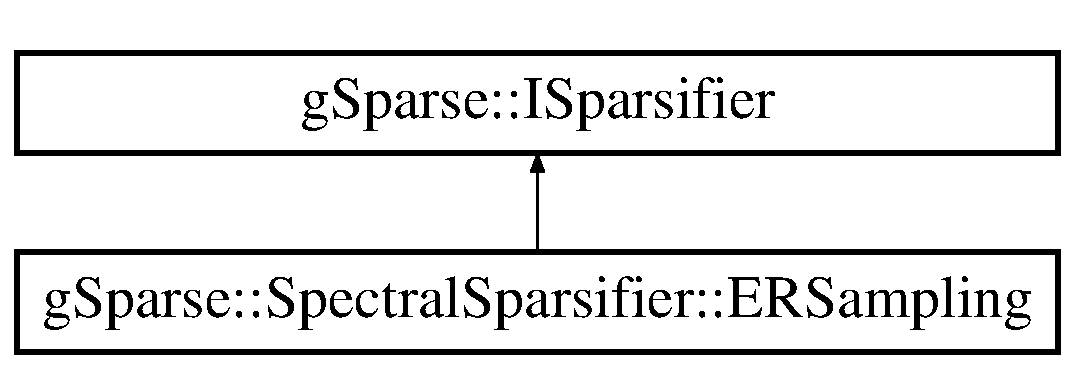
\includegraphics[height=2.000000cm]{classg_sparse_1_1_i_sparsifier}
\end{center}
\end{figure}
\subsection*{Public Member Functions}
\begin{DoxyCompactItemize}
\item 
\mbox{\Hypertarget{classg_sparse_1_1_i_sparsifier_a06f2be6951ef90ec695cadf57ce2cb3e}\label{classg_sparse_1_1_i_sparsifier_a06f2be6951ef90ec695cadf57ce2cb3e}} 
virtual C\+O\+M\+P\+U\+T\+E\+\_\+\+I\+N\+FO \mbox{\hyperlink{classg_sparse_1_1_i_sparsifier_a06f2be6951ef90ec695cadf57ce2cb3e}{Compute}} ()=0
\begin{DoxyCompactList}\small\item\em A pure virtual member to computer sparsifier weight. \end{DoxyCompactList}\item 
\mbox{\Hypertarget{classg_sparse_1_1_i_sparsifier_ad69f4c1fed9c6bc8778b716885f8fe04}\label{classg_sparse_1_1_i_sparsifier_ad69f4c1fed9c6bc8778b716885f8fe04}} 
virtual C\+O\+M\+P\+U\+T\+E\+\_\+\+I\+N\+FO \mbox{\hyperlink{classg_sparse_1_1_i_sparsifier_ad69f4c1fed9c6bc8778b716885f8fe04}{Get\+Info}} () const =0
\begin{DoxyCompactList}\small\item\em A pure virtual member to get computation status of Sparsifier. \end{DoxyCompactList}\item 
\mbox{\Hypertarget{classg_sparse_1_1_i_sparsifier_a2e1abc3830d561366a0c0e1477510c63}\label{classg_sparse_1_1_i_sparsifier_a2e1abc3830d561366a0c0e1477510c63}} 
virtual g\+Sparse\+::\+Graph \mbox{\hyperlink{classg_sparse_1_1_i_sparsifier_a2e1abc3830d561366a0c0e1477510c63}{Get\+Sparsified\+Graph}} ()=0
\begin{DoxyCompactList}\small\item\em A pure virtual member to sparsifier a graph. \end{DoxyCompactList}\end{DoxyCompactItemize}


\subsection{Detailed Description}
An interface class for Graph Sparsifier. 

This class defines an interface for g\+Sparse\textquotesingle{}s Sparsifier 

The documentation for this class was generated from the following file\+:\begin{DoxyCompactItemize}
\item 
/\+Users/\+Bomb/\+Documents/\+Project/g\+Sparse/include/g\+Sparse/\+Interface/Sparsifier.\+hpp\end{DoxyCompactItemize}

\hypertarget{classg_sparse_1_1_undirected_graph}{}\section{g\+Sparse\+:\+:Undirected\+Graph Class Reference}
\label{classg_sparse_1_1_undirected_graph}\index{g\+Sparse\+::\+Undirected\+Graph@{g\+Sparse\+::\+Undirected\+Graph}}


An Undirected Graph class.  




{\ttfamily \#include $<$Undirected\+Graph.\+hpp$>$}

Inheritance diagram for g\+Sparse\+:\+:Undirected\+Graph\+:\begin{figure}[H]
\begin{center}
\leavevmode
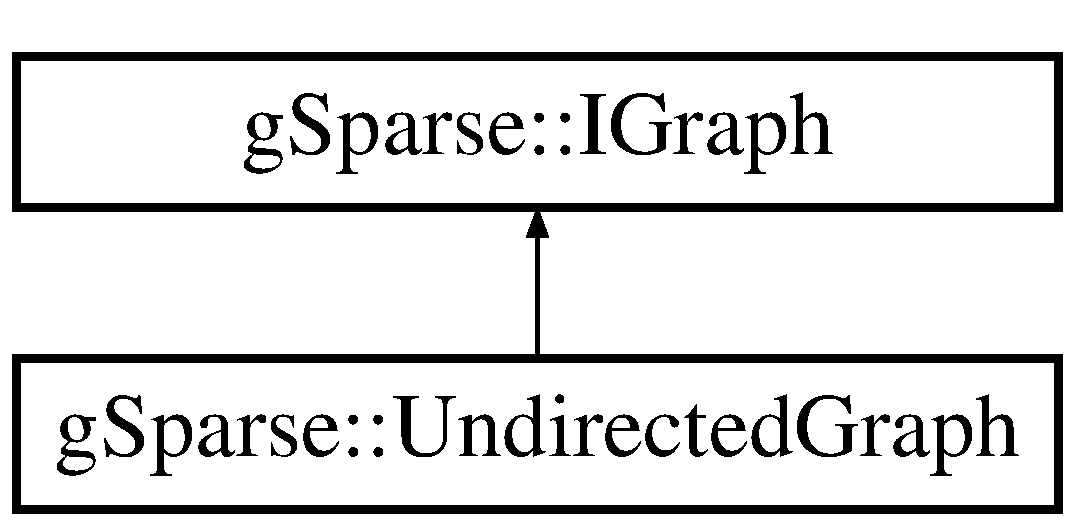
\includegraphics[height=2.000000cm]{classg_sparse_1_1_undirected_graph}
\end{center}
\end{figure}
\subsection*{Public Member Functions}
\begin{DoxyCompactItemize}
\item 
\mbox{\Hypertarget{classg_sparse_1_1_undirected_graph_a2e8177317d83d7a468c4abd69dcf3bb1}\label{classg_sparse_1_1_undirected_graph_a2e8177317d83d7a468c4abd69dcf3bb1}} 
\mbox{\hyperlink{classg_sparse_1_1_undirected_graph_a2e8177317d83d7a468c4abd69dcf3bb1}{Undirected\+Graph}} (const \mbox{\hyperlink{classg_sparse_1_1_undirected_graph}{Undirected\+Graph}} \&graph)=delete
\begin{DoxyCompactList}\small\item\em Graph data type should not be copied by value. \end{DoxyCompactList}\item 
\mbox{\Hypertarget{classg_sparse_1_1_undirected_graph_a1861d653adafc04d227819603de7e446}\label{classg_sparse_1_1_undirected_graph_a1861d653adafc04d227819603de7e446}} 
\mbox{\hyperlink{classg_sparse_1_1_undirected_graph}{Undirected\+Graph}} \& \mbox{\hyperlink{classg_sparse_1_1_undirected_graph_a1861d653adafc04d227819603de7e446}{operator=}} (const \mbox{\hyperlink{classg_sparse_1_1_undirected_graph}{Undirected\+Graph}} \&rhs)=delete
\begin{DoxyCompactList}\small\item\em Graph data type should not be copied by value / reassigne due to Eigen data type. \end{DoxyCompactList}\item 
\mbox{\hyperlink{classg_sparse_1_1_undirected_graph_a3f87a642cb86f46a6a53434598cc1674}{Undirected\+Graph}} (const g\+Sparse\+::\+Graph\+Reader \&Data\+Reader)
\begin{DoxyCompactList}\small\item\em A constructor to initialize graph based on Graph\+Reader. \end{DoxyCompactList}\item 
\mbox{\hyperlink{classg_sparse_1_1_undirected_graph_ad9dcd1dd5a47a1f35ee019a007e3cc40}{Undirected\+Graph}} (const g\+Sparse\+::\+Edge\+Matrix \&Edges)
\begin{DoxyCompactList}\small\item\em A constructor to initialize graph based from Edge data. Weight sets to one. \end{DoxyCompactList}\item 
\mbox{\hyperlink{classg_sparse_1_1_undirected_graph_af9609f1e66af95a0bf201a1185394421}{Undirected\+Graph}} (const g\+Sparse\+::\+Edge\+Matrix \&Edges, const g\+Sparse\+::\+Precision\+Row\+Matrix \&Weights)
\begin{DoxyCompactList}\small\item\em A constructor to initialize graph based from Edge data. Weight sets to one. \end{DoxyCompactList}\item 
\mbox{\Hypertarget{classg_sparse_1_1_undirected_graph_a7da2614a0e2d08d0db333b33805653a5}\label{classg_sparse_1_1_undirected_graph_a7da2614a0e2d08d0db333b33805653a5}} 
virtual const g\+Sparse\+::\+Sparse\+Precision\+Matrix \& \mbox{\hyperlink{classg_sparse_1_1_undirected_graph_a7da2614a0e2d08d0db333b33805653a5}{Get\+Adjacent\+Matrix}} () const
\begin{DoxyCompactList}\small\item\em Return Graph\textquotesingle{}s Adjancency Matrix. \end{DoxyCompactList}\item 
\mbox{\Hypertarget{classg_sparse_1_1_undirected_graph_a27df92e35ec3268554cf90b8d338e239}\label{classg_sparse_1_1_undirected_graph_a27df92e35ec3268554cf90b8d338e239}} 
virtual const g\+Sparse\+::\+Sparse\+Precision\+Matrix \& \mbox{\hyperlink{classg_sparse_1_1_undirected_graph_a27df92e35ec3268554cf90b8d338e239}{Get\+Incident\+Matrix}} () const
\begin{DoxyCompactList}\small\item\em Return Graph\textquotesingle{}s Incident Matrix. \end{DoxyCompactList}\item 
\mbox{\Hypertarget{classg_sparse_1_1_undirected_graph_a5d4e1c4a7954d963042e07f59148bda8}\label{classg_sparse_1_1_undirected_graph_a5d4e1c4a7954d963042e07f59148bda8}} 
virtual const g\+Sparse\+::\+Sparse\+Precision\+Matrix \& \mbox{\hyperlink{classg_sparse_1_1_undirected_graph_a5d4e1c4a7954d963042e07f59148bda8}{Get\+Degree\+Matrix}} () const
\begin{DoxyCompactList}\small\item\em Return Graph\textquotesingle{}s Degree Matrix. \end{DoxyCompactList}\item 
\mbox{\Hypertarget{classg_sparse_1_1_undirected_graph_a0cc819ed304d93041444ae34dd70c4ca}\label{classg_sparse_1_1_undirected_graph_a0cc819ed304d93041444ae34dd70c4ca}} 
virtual const g\+Sparse\+::\+Sparse\+Precision\+Matrix \& \mbox{\hyperlink{classg_sparse_1_1_undirected_graph_a0cc819ed304d93041444ae34dd70c4ca}{Get\+Weight\+Matrix}} () const
\begin{DoxyCompactList}\small\item\em Return Graph\textquotesingle{}s Weight Matrix. \end{DoxyCompactList}\item 
\mbox{\Hypertarget{classg_sparse_1_1_undirected_graph_a6587d7e4e37961469f26b1d5f9ae66cc}\label{classg_sparse_1_1_undirected_graph_a6587d7e4e37961469f26b1d5f9ae66cc}} 
virtual const g\+Sparse\+::\+Sparse\+Precision\+Matrix \& \mbox{\hyperlink{classg_sparse_1_1_undirected_graph_a6587d7e4e37961469f26b1d5f9ae66cc}{Get\+Laplacian\+Matrix}} () const
\begin{DoxyCompactList}\small\item\em Return Graph\textquotesingle{}s Laplacian Matrix. \end{DoxyCompactList}\item 
\mbox{\Hypertarget{classg_sparse_1_1_undirected_graph_a1e895346411557dc8a52843c279bddee}\label{classg_sparse_1_1_undirected_graph_a1e895346411557dc8a52843c279bddee}} 
virtual const g\+Sparse\+::\+Edge\+Matrix \& \mbox{\hyperlink{classg_sparse_1_1_undirected_graph_a1e895346411557dc8a52843c279bddee}{Get\+Edge\+List}} () const
\begin{DoxyCompactList}\small\item\em Return Graph\textquotesingle{}s Edge List Matrix. \end{DoxyCompactList}\item 
\mbox{\Hypertarget{classg_sparse_1_1_undirected_graph_a61a27ee51b72dc55ec3699222108af73}\label{classg_sparse_1_1_undirected_graph_a61a27ee51b72dc55ec3699222108af73}} 
virtual const g\+Sparse\+::\+Precision\+Row\+Matrix \& \mbox{\hyperlink{classg_sparse_1_1_undirected_graph_a61a27ee51b72dc55ec3699222108af73}{Get\+Weight\+List}} () const
\begin{DoxyCompactList}\small\item\em Return Graph\textquotesingle{}s Weight List Matrix. \end{DoxyCompactList}\item 
\mbox{\Hypertarget{classg_sparse_1_1_undirected_graph_a31402a2e8a8de8392720ed65a5ebb704}\label{classg_sparse_1_1_undirected_graph_a31402a2e8a8de8392720ed65a5ebb704}} 
virtual std\+::size\+\_\+t \mbox{\hyperlink{classg_sparse_1_1_undirected_graph_a31402a2e8a8de8392720ed65a5ebb704}{Get\+Edge\+Count}} () const
\begin{DoxyCompactList}\small\item\em Return the number of Edges in the Graph. \end{DoxyCompactList}\item 
\mbox{\Hypertarget{classg_sparse_1_1_undirected_graph_abd69914de28b291a6e454b39359eedc3}\label{classg_sparse_1_1_undirected_graph_abd69914de28b291a6e454b39359eedc3}} 
virtual std\+::size\+\_\+t \mbox{\hyperlink{classg_sparse_1_1_undirected_graph_abd69914de28b291a6e454b39359eedc3}{Get\+Node\+Count}} () const
\begin{DoxyCompactList}\small\item\em Return the number of Nodes in the Graph. \end{DoxyCompactList}\end{DoxyCompactItemize}
\subsection*{Protected Attributes}
\begin{DoxyCompactItemize}
\item 
\mbox{\Hypertarget{classg_sparse_1_1_undirected_graph_ae1365f68c3d3432e0bd538e1355be667}\label{classg_sparse_1_1_undirected_graph_ae1365f68c3d3432e0bd538e1355be667}} 
g\+Sparse\+::\+Sparse\+Precision\+Matrix \mbox{\hyperlink{classg_sparse_1_1_undirected_graph_ae1365f68c3d3432e0bd538e1355be667}{\+\_\+adj\+Matrix}}
\begin{DoxyCompactList}\small\item\em adjacency matrix representation \end{DoxyCompactList}\item 
\mbox{\Hypertarget{classg_sparse_1_1_undirected_graph_a4633cf520000c5aa4640768d0321cc4c}\label{classg_sparse_1_1_undirected_graph_a4633cf520000c5aa4640768d0321cc4c}} 
g\+Sparse\+::\+Sparse\+Precision\+Matrix \mbox{\hyperlink{classg_sparse_1_1_undirected_graph_a4633cf520000c5aa4640768d0321cc4c}{\+\_\+deg\+Matrix}}
\begin{DoxyCompactList}\small\item\em degree matrix representation \end{DoxyCompactList}\item 
\mbox{\Hypertarget{classg_sparse_1_1_undirected_graph_a5b666ae29ef80014ca85ca9bbde83727}\label{classg_sparse_1_1_undirected_graph_a5b666ae29ef80014ca85ca9bbde83727}} 
g\+Sparse\+::\+Sparse\+Precision\+Matrix \mbox{\hyperlink{classg_sparse_1_1_undirected_graph_a5b666ae29ef80014ca85ca9bbde83727}{\+\_\+incident\+Matrix}}
\begin{DoxyCompactList}\small\item\em incident matrix representation \end{DoxyCompactList}\item 
\mbox{\Hypertarget{classg_sparse_1_1_undirected_graph_ae84602486ec10f1c09721417e85afcb0}\label{classg_sparse_1_1_undirected_graph_ae84602486ec10f1c09721417e85afcb0}} 
g\+Sparse\+::\+Sparse\+Precision\+Matrix \mbox{\hyperlink{classg_sparse_1_1_undirected_graph_ae84602486ec10f1c09721417e85afcb0}{\+\_\+weight\+Matrix}}
\begin{DoxyCompactList}\small\item\em weight matrix representation \end{DoxyCompactList}\item 
\mbox{\Hypertarget{classg_sparse_1_1_undirected_graph_aafd3eaa27352e7f6f282e788717c2db3}\label{classg_sparse_1_1_undirected_graph_aafd3eaa27352e7f6f282e788717c2db3}} 
g\+Sparse\+::\+Sparse\+Precision\+Matrix \mbox{\hyperlink{classg_sparse_1_1_undirected_graph_aafd3eaa27352e7f6f282e788717c2db3}{\+\_\+laplacian\+Matrix}}
\begin{DoxyCompactList}\small\item\em laplacian matrix representation \end{DoxyCompactList}\item 
\mbox{\Hypertarget{classg_sparse_1_1_undirected_graph_a19665449e89f16fc75cdee3c165f3c47}\label{classg_sparse_1_1_undirected_graph_a19665449e89f16fc75cdee3c165f3c47}} 
g\+Sparse\+::\+Edge\+Matrix \mbox{\hyperlink{classg_sparse_1_1_undirected_graph_a19665449e89f16fc75cdee3c165f3c47}{\+\_\+edges}}
\begin{DoxyCompactList}\small\item\em edge list \end{DoxyCompactList}\item 
\mbox{\Hypertarget{classg_sparse_1_1_undirected_graph_a89a63f601898c7bf5342632a919ce4a4}\label{classg_sparse_1_1_undirected_graph_a89a63f601898c7bf5342632a919ce4a4}} 
g\+Sparse\+::\+Precision\+Row\+Matrix \mbox{\hyperlink{classg_sparse_1_1_undirected_graph_a89a63f601898c7bf5342632a919ce4a4}{\+\_\+weights}}
\begin{DoxyCompactList}\small\item\em weight list \end{DoxyCompactList}\item 
\mbox{\Hypertarget{classg_sparse_1_1_undirected_graph_ab10bc8ab3defed1dae0ecf2438d1022e}\label{classg_sparse_1_1_undirected_graph_ab10bc8ab3defed1dae0ecf2438d1022e}} 
std\+::size\+\_\+t \mbox{\hyperlink{classg_sparse_1_1_undirected_graph_ab10bc8ab3defed1dae0ecf2438d1022e}{\+\_\+edge\+Count}}
\begin{DoxyCompactList}\small\item\em count of edges \end{DoxyCompactList}\item 
\mbox{\Hypertarget{classg_sparse_1_1_undirected_graph_a800146dca9f76f0b55a2f4e19d7016fc}\label{classg_sparse_1_1_undirected_graph_a800146dca9f76f0b55a2f4e19d7016fc}} 
std\+::size\+\_\+t \mbox{\hyperlink{classg_sparse_1_1_undirected_graph_a800146dca9f76f0b55a2f4e19d7016fc}{\+\_\+node\+Count}}
\begin{DoxyCompactList}\small\item\em number of vertices \end{DoxyCompactList}\end{DoxyCompactItemize}
\subsection*{Additional Inherited Members}


\subsection{Detailed Description}
An Undirected Graph class. 

This class provides a multiple representation of an Undirected, Simple graph. 

\subsection{Constructor \& Destructor Documentation}
\mbox{\Hypertarget{classg_sparse_1_1_undirected_graph_a3f87a642cb86f46a6a53434598cc1674}\label{classg_sparse_1_1_undirected_graph_a3f87a642cb86f46a6a53434598cc1674}} 
\index{g\+Sparse\+::\+Undirected\+Graph@{g\+Sparse\+::\+Undirected\+Graph}!Undirected\+Graph@{Undirected\+Graph}}
\index{Undirected\+Graph@{Undirected\+Graph}!g\+Sparse\+::\+Undirected\+Graph@{g\+Sparse\+::\+Undirected\+Graph}}
\subsubsection{\texorpdfstring{Undirected\+Graph()}{UndirectedGraph()}\hspace{0.1cm}{\footnotesize\ttfamily [1/3]}}
{\footnotesize\ttfamily g\+Sparse\+::\+Undirected\+Graph\+::\+Undirected\+Graph (\begin{DoxyParamCaption}\item[{const g\+Sparse\+::\+Graph\+Reader \&}]{Data\+Reader }\end{DoxyParamCaption})\hspace{0.3cm}{\ttfamily [inline]}}



A constructor to initialize graph based on Graph\+Reader. 


\begin{DoxyParams}{Parameters}
{\em Data\+Reader} & A subclass of \mbox{\hyperlink{classg_sparse_1_1_i_graph_reader}{I\+Graph\+Reader}} which provides an interface to read external data. \\
\hline
\end{DoxyParams}
\mbox{\Hypertarget{classg_sparse_1_1_undirected_graph_ad9dcd1dd5a47a1f35ee019a007e3cc40}\label{classg_sparse_1_1_undirected_graph_ad9dcd1dd5a47a1f35ee019a007e3cc40}} 
\index{g\+Sparse\+::\+Undirected\+Graph@{g\+Sparse\+::\+Undirected\+Graph}!Undirected\+Graph@{Undirected\+Graph}}
\index{Undirected\+Graph@{Undirected\+Graph}!g\+Sparse\+::\+Undirected\+Graph@{g\+Sparse\+::\+Undirected\+Graph}}
\subsubsection{\texorpdfstring{Undirected\+Graph()}{UndirectedGraph()}\hspace{0.1cm}{\footnotesize\ttfamily [2/3]}}
{\footnotesize\ttfamily g\+Sparse\+::\+Undirected\+Graph\+::\+Undirected\+Graph (\begin{DoxyParamCaption}\item[{const g\+Sparse\+::\+Edge\+Matrix \&}]{Edges }\end{DoxyParamCaption})\hspace{0.3cm}{\ttfamily [inline]}}



A constructor to initialize graph based from Edge data. Weight sets to one. 


\begin{DoxyParams}{Parameters}
{\em Edges} & An Eigen Matrix containing Edge List. \\
\hline
\end{DoxyParams}
\mbox{\Hypertarget{classg_sparse_1_1_undirected_graph_af9609f1e66af95a0bf201a1185394421}\label{classg_sparse_1_1_undirected_graph_af9609f1e66af95a0bf201a1185394421}} 
\index{g\+Sparse\+::\+Undirected\+Graph@{g\+Sparse\+::\+Undirected\+Graph}!Undirected\+Graph@{Undirected\+Graph}}
\index{Undirected\+Graph@{Undirected\+Graph}!g\+Sparse\+::\+Undirected\+Graph@{g\+Sparse\+::\+Undirected\+Graph}}
\subsubsection{\texorpdfstring{Undirected\+Graph()}{UndirectedGraph()}\hspace{0.1cm}{\footnotesize\ttfamily [3/3]}}
{\footnotesize\ttfamily g\+Sparse\+::\+Undirected\+Graph\+::\+Undirected\+Graph (\begin{DoxyParamCaption}\item[{const g\+Sparse\+::\+Edge\+Matrix \&}]{Edges,  }\item[{const g\+Sparse\+::\+Precision\+Row\+Matrix \&}]{Weights }\end{DoxyParamCaption})\hspace{0.3cm}{\ttfamily [inline]}}



A constructor to initialize graph based from Edge data. Weight sets to one. 


\begin{DoxyParams}{Parameters}
{\em Edges} & An Eigen Matrix containing Edge List. \\
\hline
{\em Weights} & An Eigen Matrix containing associated Weights. \\
\hline
\end{DoxyParams}


The documentation for this class was generated from the following file\+:\begin{DoxyCompactItemize}
\item 
/\+Users/\+Bomb/\+Documents/\+Project/g\+Sparse/include/g\+Sparse/Undirected\+Graph.\+hpp\end{DoxyCompactItemize}

%--- End generated contents ---

% Index
\backmatter
\newpage
\phantomsection
\clearemptydoublepage
\addcontentsline{toc}{chapter}{Index}
\printindex

\end{document}
